\documentclass{book}
\usepackage[a4paper,top=2.5cm,bottom=2.5cm,left=2.5cm,right=2.5cm]{geometry}
\usepackage{makeidx}
\usepackage{natbib}
\usepackage{graphicx}
\usepackage{multicol}
\usepackage{float}
\usepackage{listings}
\usepackage{color}
\usepackage{ifthen}
\usepackage[table]{xcolor}
\usepackage{textcomp}
\usepackage{alltt}
\usepackage{ifpdf}
\ifpdf
\usepackage[pdftex,
            pagebackref=true,
            colorlinks=true,
            linkcolor=blue,
            unicode
           ]{hyperref}
\else
\usepackage[ps2pdf,
            pagebackref=true,
            colorlinks=true,
            linkcolor=blue,
            unicode
           ]{hyperref}
\usepackage{pspicture}
\fi
\usepackage[utf8]{inputenc}
\usepackage[french]{babel}

\usepackage{mathptmx}
\usepackage[scaled=.90]{helvet}
\usepackage{courier}
\usepackage{sectsty}
\usepackage{amssymb}
\usepackage[titles]{tocloft}
\usepackage{doxygen}
\lstset{language=C++,inputencoding=utf8,basicstyle=\footnotesize,breaklines=true,breakatwhitespace=true,tabsize=8,numbers=left }
\makeindex
\setcounter{tocdepth}{3}
\renewcommand{\footrulewidth}{0.4pt}
\renewcommand{\familydefault}{\sfdefault}
\hfuzz=15pt
\setlength{\emergencystretch}{15pt}
\hbadness=750
\tolerance=750
\begin{document}
\hypersetup{pageanchor=false,citecolor=blue}
\begin{titlepage}
\vspace*{7cm}
\begin{center}
{\Large S\-Y\-S -\/ Petits Chevaux }\\
\vspace*{1cm}
{\large Généré par Doxygen 1.8.1.2}\\
\vspace*{0.5cm}
{\small Jeudi Octobre 23 2014 16:24:26}\\
\end{center}
\end{titlepage}
\clearemptydoublepage
\pagenumbering{roman}
\tableofcontents
\clearemptydoublepage
\pagenumbering{arabic}
\hypersetup{pageanchor=true,citecolor=blue}
\chapter{Index des structures de données}
\section{Structures de données}
Liste des structures de données avec une brève description \-:\begin{DoxyCompactList}
\item\contentsline{section}{\hyperlink{structstruct__debuttour}{struct\-\_\-debuttour} \\*Informations transmises par le pere pour les joueurs en debut de tour }{\pageref{structstruct__debuttour}}{}
\item\contentsline{section}{\hyperlink{structstruct__pendantjeu}{struct\-\_\-pendantjeu} \\*Informations transmises par les joueurs pour les autres joueurs pendant le tour }{\pageref{structstruct__pendantjeu}}{}
\item\contentsline{section}{\hyperlink{structstruct__retourjeu}{struct\-\_\-retourjeu} \\*Informations transmises par les joueurs pour le pere en fin de tour }{\pageref{structstruct__retourjeu}}{}
\end{DoxyCompactList}

\chapter{Index des fichiers}
\section{Liste des fichiers}
Liste de tous les fichiers avec une brève description \-:\begin{DoxyCompactList}
\item\contentsline{section}{src/\hyperlink{dada_8c}{dada.\-c} \\*Programme de jeu des petits chevaux utilisant des fork() et des pipes }{\pageref{dada_8c}}{}
\item\contentsline{section}{src/\hyperlink{des_8c}{des.\-c} \\*Fonctions de simulation d'un tirage de des }{\pageref{des_8c}}{}
\item\contentsline{section}{src/\hyperlink{jeu_8c}{jeu.\-c} \\*Fonctions relatives au jeu pour le programme Petits Chevaux }{\pageref{jeu_8c}}{}
\item\contentsline{section}{src/\hyperlink{pipes_8c}{pipes.\-c} \\*Fonctions relatives au pipes pour le jeu Petits chevaux }{\pageref{pipes_8c}}{}
\item\contentsline{section}{src/\hyperlink{regles_8c}{regles.\-c} \\*Fonctions relatives aux regles pour le jeu Petits chevaux }{\pageref{regles_8c}}{}
\item\contentsline{section}{src/headers/\hyperlink{dada_8h}{dada.\-h} \\*Declaration des fonctions de verification pour la lecture/ecriture dans les pipes }{\pageref{dada_8h}}{}
\item\contentsline{section}{src/headers/\hyperlink{des_8h}{des.\-h} \\*Declaration des fonctions relatives au des pour le jeu Petits chevaux }{\pageref{des_8h}}{}
\item\contentsline{section}{src/headers/\hyperlink{jeu_8h}{jeu.\-h} \\*Declaration des fonctions relatives au jeu pour le jeu Petits chevaux }{\pageref{jeu_8h}}{}
\item\contentsline{section}{src/headers/\hyperlink{pipes_8h}{pipes.\-h} \\*Declaration des fonctions relatives au pipes pour le jeu Petits chevaux }{\pageref{pipes_8h}}{}
\item\contentsline{section}{src/headers/\hyperlink{regles_8h}{regles.\-h} \\*Declaration des fonctions relatives aux regles pour le jeu Petits chevaux }{\pageref{regles_8h}}{}
\end{DoxyCompactList}

\chapter{Documentation des structures de données}
\hypertarget{structstruct__debuttour}{\section{Référence de la structure struct\-\_\-debuttour}
\label{structstruct__debuttour}\index{struct\-\_\-debuttour@{struct\-\_\-debuttour}}
}


Informations transmises par le pere pour les joueurs en debut de tour.  




{\ttfamily \#include $<$jeu.\-h$>$}

\subsection*{Champs de données}
\begin{DoxyCompactItemize}
\item 
int \hyperlink{structstruct__debuttour_ae1ce459099bf548d3ae61f39c892ebbe}{partieencours}
\item 
int \hyperlink{structstruct__debuttour_a3e4028dc4a9077afc6e53e423343bd70}{numerojoueur}
\end{DoxyCompactItemize}


\subsection{Description détaillée}
Informations transmises par le pere pour les joueurs en debut de tour. 

partieencours vaut 1 tant que la partie est en cours. Sinon 0. numerojoueur correspond au numero du joueur devant jouer au prochain tour 

\subsection{Documentation des champs}
\hypertarget{structstruct__debuttour_a3e4028dc4a9077afc6e53e423343bd70}{\index{struct\-\_\-debuttour@{struct\-\_\-debuttour}!numerojoueur@{numerojoueur}}
\index{numerojoueur@{numerojoueur}!struct_debuttour@{struct\-\_\-debuttour}}
\subsubsection[{numerojoueur}]{\setlength{\rightskip}{0pt plus 5cm}int numerojoueur}}\label{structstruct__debuttour_a3e4028dc4a9077afc6e53e423343bd70}
Numero du joueur devant jouer au prochain tour \hypertarget{structstruct__debuttour_ae1ce459099bf548d3ae61f39c892ebbe}{\index{struct\-\_\-debuttour@{struct\-\_\-debuttour}!partieencours@{partieencours}}
\index{partieencours@{partieencours}!struct_debuttour@{struct\-\_\-debuttour}}
\subsubsection[{partieencours}]{\setlength{\rightskip}{0pt plus 5cm}int partieencours}}\label{structstruct__debuttour_ae1ce459099bf548d3ae61f39c892ebbe}
Indique si la partie est encors en cours 1. Sinon 0 

La documentation de cette structure a été générée à partir du fichier suivant \-:\begin{DoxyCompactItemize}
\item 
src/headers/\hyperlink{jeu_8h}{jeu.\-h}\end{DoxyCompactItemize}

\hypertarget{structstruct__pendantjeu}{\section{Référence de la structure struct\-\_\-pendantjeu}
\label{structstruct__pendantjeu}\index{struct\-\_\-pendantjeu@{struct\-\_\-pendantjeu}}
}


Informations transmises par les joueurs pour les autres joueurs pendant le tour.  




{\ttfamily \#include $<$jeu.\-h$>$}

\subsection*{Champs de données}
\begin{DoxyCompactItemize}
\item 
int \hyperlink{structstruct__pendantjeu_a3e4028dc4a9077afc6e53e423343bd70}{numerojoueur}
\item 
int \hyperlink{structstruct__pendantjeu_a886601c5a72273d41b31c90740071a61}{positionjoueur}
\end{DoxyCompactItemize}


\subsection{Description détaillée}
Informations transmises par les joueurs pour les autres joueurs pendant le tour. 

Définition à la ligne 40 du fichier jeu.\-h.



\subsection{Documentation des champs}
\hypertarget{structstruct__pendantjeu_a3e4028dc4a9077afc6e53e423343bd70}{\index{struct\-\_\-pendantjeu@{struct\-\_\-pendantjeu}!numerojoueur@{numerojoueur}}
\index{numerojoueur@{numerojoueur}!struct_pendantjeu@{struct\-\_\-pendantjeu}}
\subsubsection[{numerojoueur}]{\setlength{\rightskip}{0pt plus 5cm}int numerojoueur}}\label{structstruct__pendantjeu_a3e4028dc4a9077afc6e53e423343bd70}
Indique le joueur venant de jouer. 

Définition à la ligne 41 du fichier jeu.\-h.

\hypertarget{structstruct__pendantjeu_a886601c5a72273d41b31c90740071a61}{\index{struct\-\_\-pendantjeu@{struct\-\_\-pendantjeu}!positionjoueur@{positionjoueur}}
\index{positionjoueur@{positionjoueur}!struct_pendantjeu@{struct\-\_\-pendantjeu}}
\subsubsection[{positionjoueur}]{\setlength{\rightskip}{0pt plus 5cm}int positionjoueur}}\label{structstruct__pendantjeu_a886601c5a72273d41b31c90740071a61}
Indique la nouvelle position de ce joueur. Utile pour faire revenir les chevaux a la case depart si deux se trouvent simultanement sur la meme case. 

Définition à la ligne 42 du fichier jeu.\-h.



La documentation de cette structure a été générée à partir du fichier suivant \-:\begin{DoxyCompactItemize}
\item 
src/headers/\hyperlink{jeu_8h}{jeu.\-h}\end{DoxyCompactItemize}

\hypertarget{structstruct__retourjeu}{\section{Référence de la structure struct\-\_\-retourjeu}
\label{structstruct__retourjeu}\index{struct\-\_\-retourjeu@{struct\-\_\-retourjeu}}
}


Informations transmises par les joueurs pour le pere en fin de tour.  




{\ttfamily \#include $<$jeu.\-h$>$}

\subsection*{Champs de données}
\begin{DoxyCompactItemize}
\item 
int \hyperlink{structstruct__retourjeu_a3e4028dc4a9077afc6e53e423343bd70}{numerojoueur}
\item 
int \hyperlink{structstruct__retourjeu_ac584e924232e3ffd27115c09c0fcc55d}{resultatde}
\item 
int \hyperlink{structstruct__retourjeu_a886601c5a72273d41b31c90740071a61}{positionjoueur}
\end{DoxyCompactItemize}


\subsection{Description détaillée}
Informations transmises par les joueurs pour le pere en fin de tour. 

\subsection{Documentation des champs}
\hypertarget{structstruct__retourjeu_a3e4028dc4a9077afc6e53e423343bd70}{\index{struct\-\_\-retourjeu@{struct\-\_\-retourjeu}!numerojoueur@{numerojoueur}}
\index{numerojoueur@{numerojoueur}!struct_retourjeu@{struct\-\_\-retourjeu}}
\subsubsection[{numerojoueur}]{\setlength{\rightskip}{0pt plus 5cm}int numerojoueur}}\label{structstruct__retourjeu_a3e4028dc4a9077afc6e53e423343bd70}
Indique le numero du joueur venant de jouer. \hypertarget{structstruct__retourjeu_a886601c5a72273d41b31c90740071a61}{\index{struct\-\_\-retourjeu@{struct\-\_\-retourjeu}!positionjoueur@{positionjoueur}}
\index{positionjoueur@{positionjoueur}!struct_retourjeu@{struct\-\_\-retourjeu}}
\subsubsection[{positionjoueur}]{\setlength{\rightskip}{0pt plus 5cm}int positionjoueur}}\label{structstruct__retourjeu_a886601c5a72273d41b31c90740071a61}
Indique la nouvelle position du joueur \hypertarget{structstruct__retourjeu_ac584e924232e3ffd27115c09c0fcc55d}{\index{struct\-\_\-retourjeu@{struct\-\_\-retourjeu}!resultatde@{resultatde}}
\index{resultatde@{resultatde}!struct_retourjeu@{struct\-\_\-retourjeu}}
\subsubsection[{resultatde}]{\setlength{\rightskip}{0pt plus 5cm}int resultatde}}\label{structstruct__retourjeu_ac584e924232e3ffd27115c09c0fcc55d}
Indique le resultat de son lance de de. Utile pour savoir si le joueur peut rejouer. 

La documentation de cette structure a été générée à partir du fichier suivant \-:\begin{DoxyCompactItemize}
\item 
src/headers/\hyperlink{jeu_8h}{jeu.\-h}\end{DoxyCompactItemize}

\chapter{Documentation des fichiers}
\hypertarget{dada_8c}{\section{Référence du fichier src/dada.c}
\label{dada_8c}\index{src/dada.\-c@{src/dada.\-c}}
}


Programme de jeu des petits chevaux utilisant des fork() et des pipes.  


{\ttfamily \#include $<$stdio.\-h$>$}\\*
{\ttfamily \#include $<$stdlib.\-h$>$}\\*
{\ttfamily \#include $<$unistd.\-h$>$}\\*
{\ttfamily \#include $<$sys/types.\-h$>$}\\*
{\ttfamily \#include $<$sys/wait.\-h$>$}\\*
{\ttfamily \#include $<$string.\-h$>$}\\*
{\ttfamily \#include \char`\"{}headers/des.\-h\char`\"{}}\\*
{\ttfamily \#include \char`\"{}headers/jeu.\-h\char`\"{}}\\*
{\ttfamily \#include \char`\"{}headers/regles.\-h\char`\"{}}\\*
{\ttfamily \#include \char`\"{}headers/pipes.\-h\char`\"{}}\\*
Graphe des dépendances par inclusion de dada.\-c\-:
\nopagebreak
\begin{figure}[H]
\begin{center}
\leavevmode
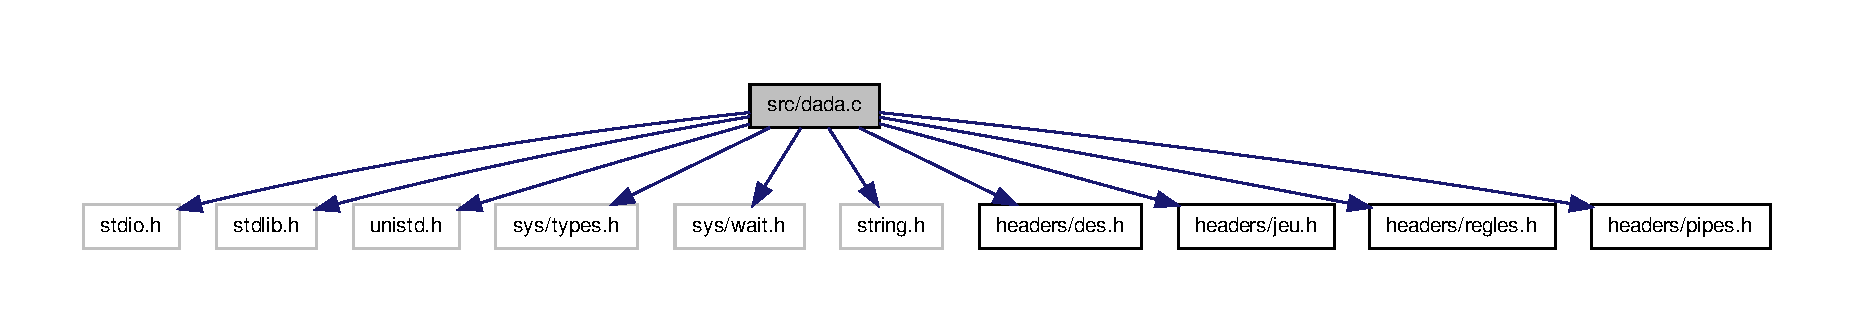
\includegraphics[width=350pt]{dada_8c__incl}
\end{center}
\end{figure}
\subsection*{Fonctions}
\begin{DoxyCompactItemize}
\item 
void \hyperlink{dada_8c_a97c9452b045a7fdb188a62e97b58e5d8}{check\-R} (int result)
\begin{DoxyCompactList}\small\item\em Fonction de verification du bon deroulement de read. \end{DoxyCompactList}\item 
void \hyperlink{dada_8c_a0f46c4e07b6faf548c663e9f8155ef48}{check\-W} (int result)
\begin{DoxyCompactList}\small\item\em Fonction de verification du bon deroulement de write. \end{DoxyCompactList}\item 
int \hyperlink{dada_8c_a0ddf1224851353fc92bfbff6f499fa97}{main} (int argc, char $\ast$argv\mbox{[}$\,$\mbox{]})
\begin{DoxyCompactList}\small\item\em Corps du programme Petit Chevaux. \end{DoxyCompactList}\end{DoxyCompactItemize}


\subsection{Description détaillée}
Programme de jeu des petits chevaux utilisant des fork() et des pipes. \begin{DoxyAuthor}{Auteur}
A\-O\-U\-N Abel et D\-O\-U\-C\-H\-E\-T Maximilien
\end{DoxyAuthor}
Fichier Principal du programme dada 

Définition dans le fichier \hyperlink{dada_8c_source}{dada.\-c}.



\subsection{Documentation des fonctions}
\hypertarget{dada_8c_a97c9452b045a7fdb188a62e97b58e5d8}{\index{dada.\-c@{dada.\-c}!check\-R@{check\-R}}
\index{check\-R@{check\-R}!dada.c@{dada.\-c}}
\subsubsection[{check\-R}]{\setlength{\rightskip}{0pt plus 5cm}void check\-R (
\begin{DoxyParamCaption}
\item[{int}]{result}
\end{DoxyParamCaption}
)}}\label{dada_8c_a97c9452b045a7fdb188a62e97b58e5d8}


Fonction de verification du bon deroulement de read. 

Fonctions de vérification pour les opérations read et write

Verifie que l'operation de lecture dans un pipe s'est bien deroulée. 
\begin{DoxyParams}{Paramètres}
{\em result} & Int -\/ Correspond au resultat de la fonction read appellée en parametre. \\
\hline
\end{DoxyParams}
\begin{DoxyReturn}{Renvoie}
Void -\/ Termine le programme en cas d'erreur 
\end{DoxyReturn}


Définition à la ligne 36 du fichier dada.\-c.



Voici le graphe des appelants de cette fonction \-:
\nopagebreak
\begin{figure}[H]
\begin{center}
\leavevmode
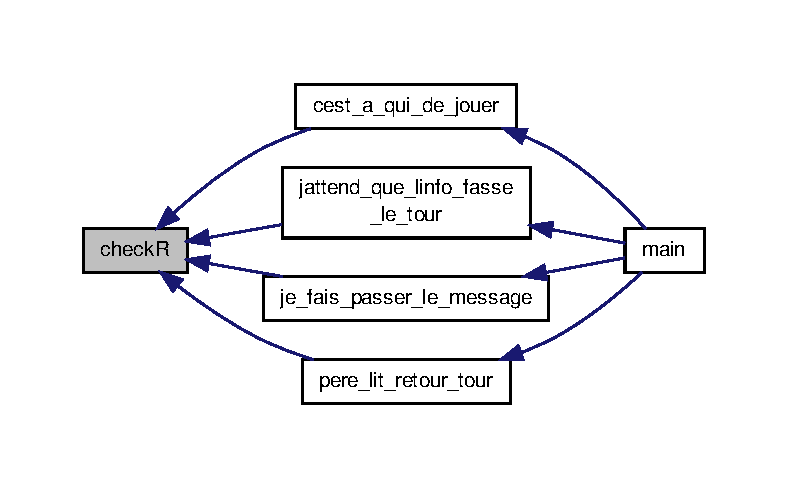
\includegraphics[width=350pt]{dada_8c_a97c9452b045a7fdb188a62e97b58e5d8_icgraph}
\end{center}
\end{figure}


\hypertarget{dada_8c_a0f46c4e07b6faf548c663e9f8155ef48}{\index{dada.\-c@{dada.\-c}!check\-W@{check\-W}}
\index{check\-W@{check\-W}!dada.c@{dada.\-c}}
\subsubsection[{check\-W}]{\setlength{\rightskip}{0pt plus 5cm}void check\-W (
\begin{DoxyParamCaption}
\item[{int}]{result}
\end{DoxyParamCaption}
)}}\label{dada_8c_a0f46c4e07b6faf548c663e9f8155ef48}


Fonction de verification du bon deroulement de write. 

Verifie que l'operation d'ecriture dans un pipe s'est bien deroulée. 
\begin{DoxyParams}{Paramètres}
{\em result} & Int -\/ Correspond au resultat de la fonction read appellée en parametre. \\
\hline
\end{DoxyParams}
\begin{DoxyReturn}{Renvoie}
Void -\/ Termine le programme en cas d'erreur 
\end{DoxyReturn}


Définition à la ligne 51 du fichier dada.\-c.



Voici le graphe des appelants de cette fonction \-:
\nopagebreak
\begin{figure}[H]
\begin{center}
\leavevmode
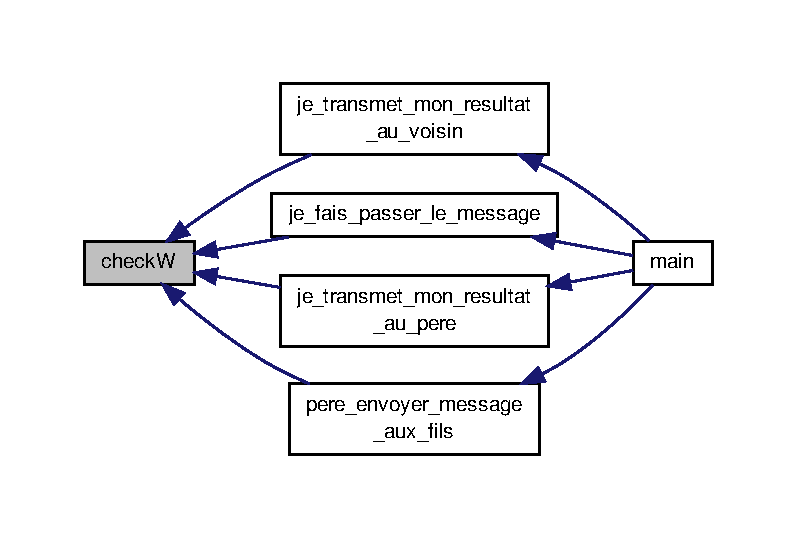
\includegraphics[width=350pt]{dada_8c_a0f46c4e07b6faf548c663e9f8155ef48_icgraph}
\end{center}
\end{figure}


\hypertarget{dada_8c_a0ddf1224851353fc92bfbff6f499fa97}{\index{dada.\-c@{dada.\-c}!main@{main}}
\index{main@{main}!dada.c@{dada.\-c}}
\subsubsection[{main}]{\setlength{\rightskip}{0pt plus 5cm}int main (
\begin{DoxyParamCaption}
\item[{int}]{argc, }
\item[{char $\ast$}]{argv\mbox{[}$\,$\mbox{]}}
\end{DoxyParamCaption}
)}}\label{dada_8c_a0ddf1224851353fc92bfbff6f499fa97}


Corps du programme Petit Chevaux. 

\begin{DoxyReturn}{Renvoie}
E\-X\-I\-T\-\_\-\-S\-U\-C\-C\-E\-S\-S -\/ Arrêt normal du programme. 
\end{DoxyReturn}
Déclaration et instanciation du tableau de pipes. Se référer à \hyperlink{pipes_8h}{pipes.\-h} pour plus d'information.

tableau des P\-I\-D de chaque fils, pid renvoyé par fork et le status renvoyé par les wait finaux

Autres variables

Pour chaque fils nous initialison une variable informant sur sa position et les structures d'informations qui vont transiter

Allocation mémoire de ces structures.

Initialisation du generateur de nombre aleatoire pour le lance de des

Création des pipes

En cas d'erreur lors de la creation du fork

Code d'execution du fils num\-\_\-fils La variable num\-\_\-fils correspond au numéro du fils en cours

Fermetures des pipes inutilises pour le fils en cours

Instanciation et initialisation de variables propres au fils num\-\_\-fils.

Corps du fils num\-\_\-fils

Fermetures des pipes restant

Code d'execution du programme principal, poursuite de la création de fils

Suite du programme principal

Fermetures des pipes inutilises

Corps du programme

Fermetures des pipes restants

Définition à la ligne 67 du fichier dada.\-c.



Voici le graphe d'appel pour cette fonction \-:
\nopagebreak
\begin{figure}[H]
\begin{center}
\leavevmode
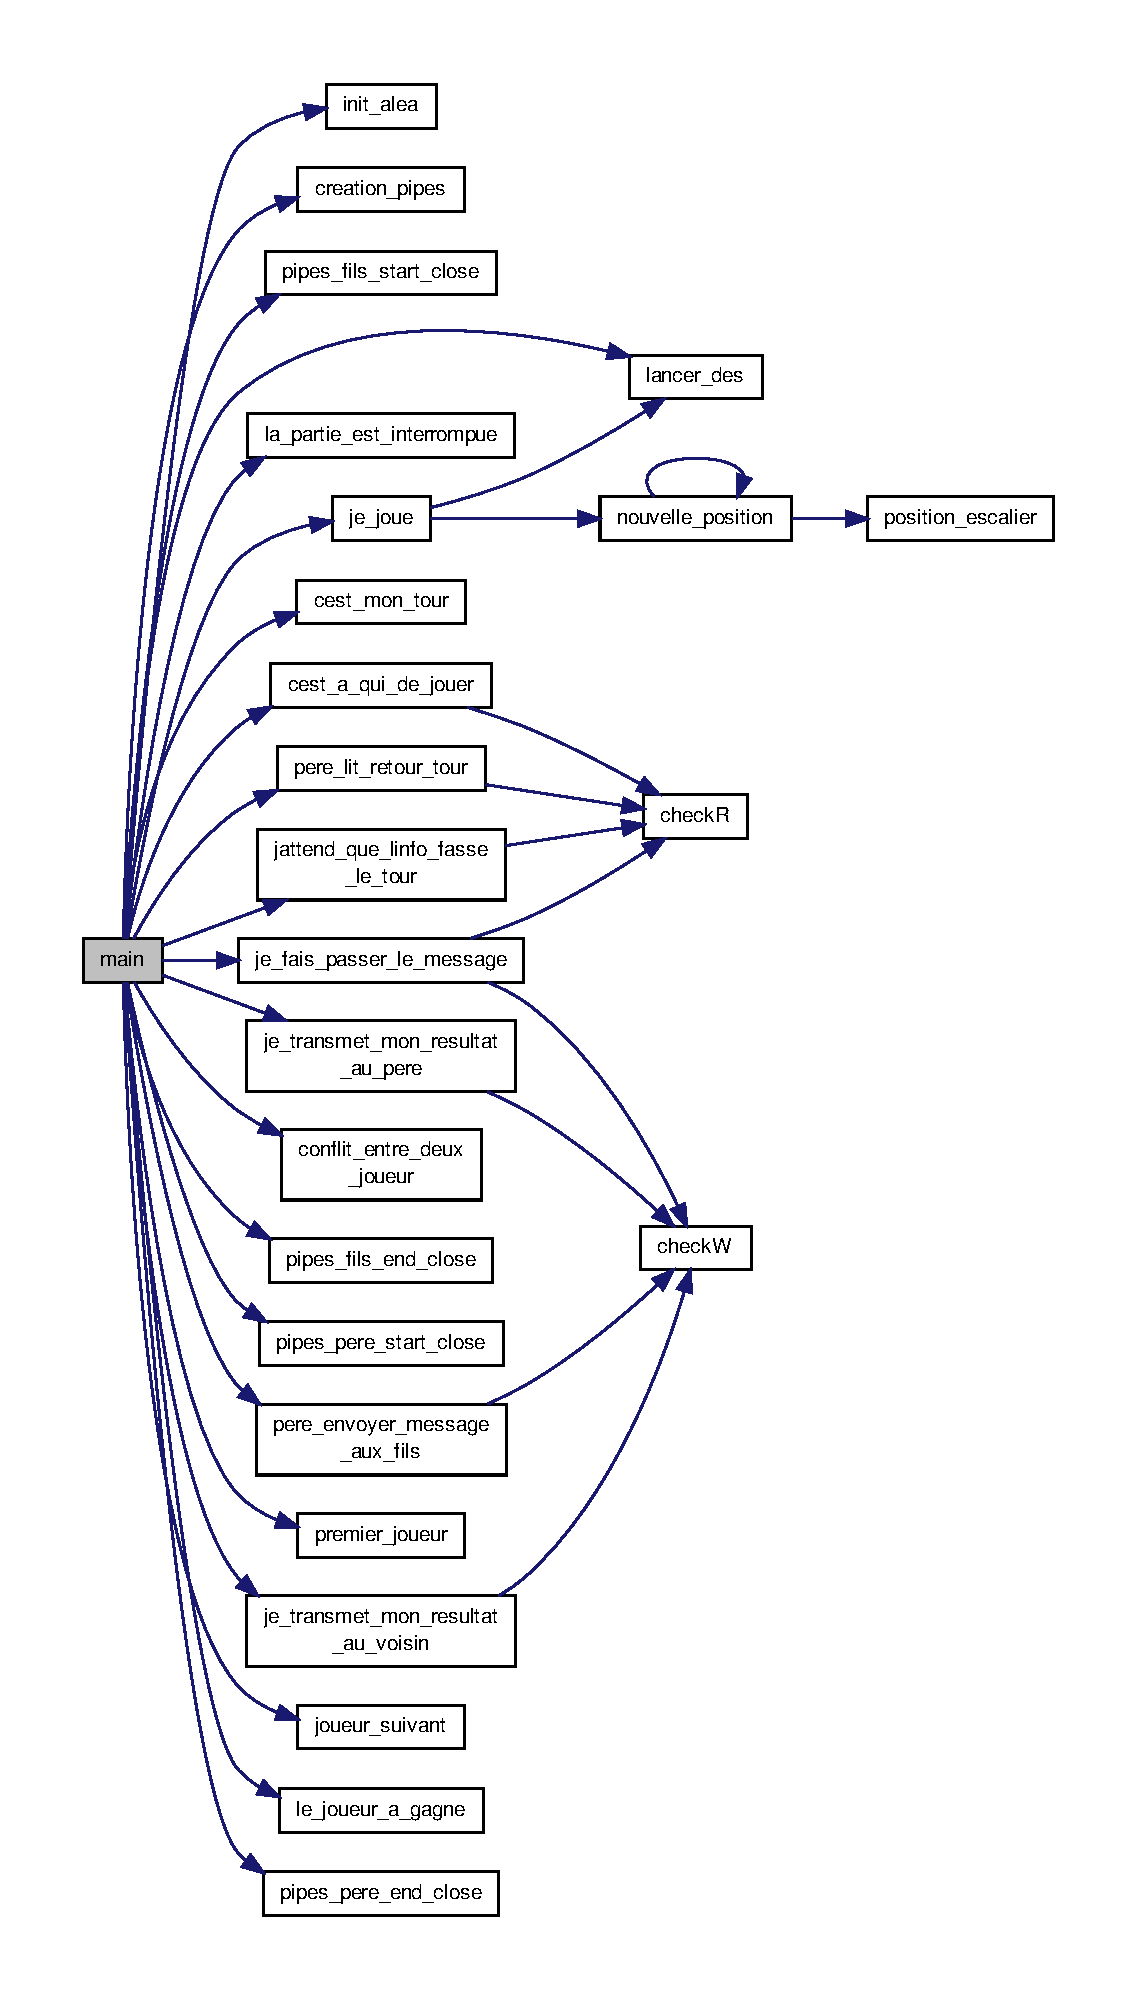
\includegraphics[height=550pt]{dada_8c_a0ddf1224851353fc92bfbff6f499fa97_cgraph}
\end{center}
\end{figure}



\hypertarget{des_8c}{\section{Référence du fichier src/des.c}
\label{des_8c}\index{src/des.\-c@{src/des.\-c}}
}


Fonctions de simulation d'un tirage de des.  


{\ttfamily \#include $<$stdlib.\-h$>$}\\*
{\ttfamily \#include $<$time.\-h$>$}\\*
Graphe des dépendances par inclusion de des.\-c\-:
\nopagebreak
\begin{figure}[H]
\begin{center}
\leavevmode
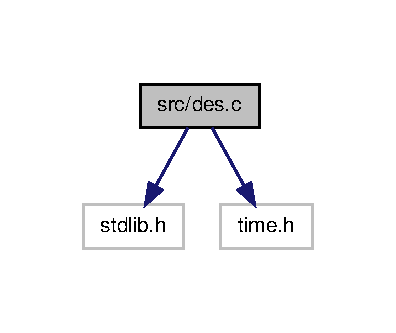
\includegraphics[width=190pt]{des_8c__incl}
\end{center}
\end{figure}
\subsection*{Fonctions}
\begin{DoxyCompactItemize}
\item 
void \hyperlink{des_8c_af951d515465516d4056cec3f4571ee28}{init\-\_\-alea} ()
\begin{DoxyCompactList}\small\item\em Initialise le generateur de nombres aleatoires. \end{DoxyCompactList}\item 
int \hyperlink{des_8c_a2d90f82862986ff270f16f9771580b53}{lancer\-\_\-des} ()
\begin{DoxyCompactList}\small\item\em Simule un lancé de dé à 6 cotés. \end{DoxyCompactList}\end{DoxyCompactItemize}


\subsection{Description détaillée}
Fonctions de simulation d'un tirage de des. \begin{DoxyAuthor}{Auteur}
A\-O\-U\-N Abel et D\-O\-U\-C\-H\-E\-T Maximilien 
\end{DoxyAuthor}


Définition dans le fichier \hyperlink{des_8c_source}{des.\-c}.



\subsection{Documentation des fonctions}
\hypertarget{des_8c_af951d515465516d4056cec3f4571ee28}{\index{des.\-c@{des.\-c}!init\-\_\-alea@{init\-\_\-alea}}
\index{init\-\_\-alea@{init\-\_\-alea}!des.c@{des.\-c}}
\subsubsection[{init\-\_\-alea}]{\setlength{\rightskip}{0pt plus 5cm}void init\-\_\-alea (
\begin{DoxyParamCaption}
{}
\end{DoxyParamCaption}
)}}\label{des_8c_af951d515465516d4056cec3f4571ee28}


Initialise le generateur de nombres aleatoires. 

Initialise la graine allant servir pour la génération de nombres aléatoire. \begin{DoxyReturn}{Renvoie}
Void 
\end{DoxyReturn}


Définition à la ligne 16 du fichier des.\-c.



Voici le graphe des appelants de cette fonction \-:
\nopagebreak
\begin{figure}[H]
\begin{center}
\leavevmode
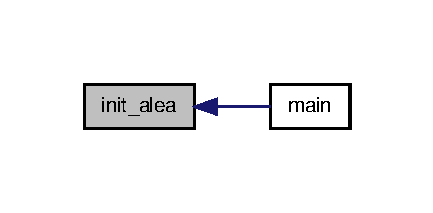
\includegraphics[width=208pt]{des_8c_af951d515465516d4056cec3f4571ee28_icgraph}
\end{center}
\end{figure}


\hypertarget{des_8c_a2d90f82862986ff270f16f9771580b53}{\index{des.\-c@{des.\-c}!lancer\-\_\-des@{lancer\-\_\-des}}
\index{lancer\-\_\-des@{lancer\-\_\-des}!des.c@{des.\-c}}
\subsubsection[{lancer\-\_\-des}]{\setlength{\rightskip}{0pt plus 5cm}int lancer\-\_\-des (
\begin{DoxyParamCaption}
{}
\end{DoxyParamCaption}
)}}\label{des_8c_a2d90f82862986ff270f16f9771580b53}


Simule un lancé de dé à 6 cotés. 

\begin{DoxyReturn}{Renvoie}
Int -\/ Compris entre 1 et 6. 
\end{DoxyReturn}


Définition à la ligne 25 du fichier des.\-c.



Voici le graphe des appelants de cette fonction \-:
\nopagebreak
\begin{figure}[H]
\begin{center}
\leavevmode
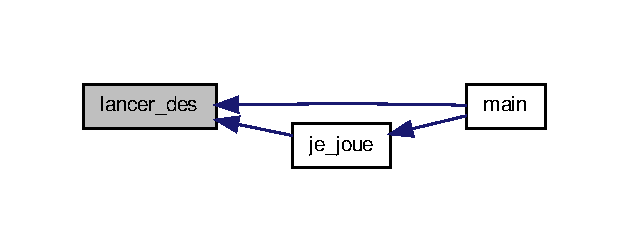
\includegraphics[width=302pt]{des_8c_a2d90f82862986ff270f16f9771580b53_icgraph}
\end{center}
\end{figure}



\hypertarget{dada_8h}{\section{Référence du fichier src/headers/dada.h}
\label{dada_8h}\index{src/headers/dada.\-h@{src/headers/dada.\-h}}
}


Declaration des fonctions de verification pour la lecture/ecriture dans les pipes.  


\subsection*{Fonctions}
\begin{DoxyCompactItemize}
\item 
void \hyperlink{dada_8h_a97c9452b045a7fdb188a62e97b58e5d8}{check\-R} (int result)
\begin{DoxyCompactList}\small\item\em Fonction de verification du bon deroulement de read. \end{DoxyCompactList}\item 
void \hyperlink{dada_8h_a0f46c4e07b6faf548c663e9f8155ef48}{check\-W} (int result)
\begin{DoxyCompactList}\small\item\em Fonction de verification du bon deroulement de write. \end{DoxyCompactList}\end{DoxyCompactItemize}


\subsection{Description détaillée}
Declaration des fonctions de verification pour la lecture/ecriture dans les pipes. \begin{DoxyAuthor}{Auteur}
A\-O\-U\-N Abel et D\-O\-U\-C\-H\-E\-T Maximilien 
\end{DoxyAuthor}


\subsection{Documentation des fonctions}
\hypertarget{dada_8h_a97c9452b045a7fdb188a62e97b58e5d8}{\index{dada.\-h@{dada.\-h}!check\-R@{check\-R}}
\index{check\-R@{check\-R}!dada.h@{dada.\-h}}
\subsubsection[{check\-R}]{\setlength{\rightskip}{0pt plus 5cm}void check\-R (
\begin{DoxyParamCaption}
\item[{int}]{result}
\end{DoxyParamCaption}
)}}\label{dada_8h_a97c9452b045a7fdb188a62e97b58e5d8}


Fonction de verification du bon deroulement de read. 

Fonctions de vérification pour les opérations read et write

Verifie que l'operation de lecture dans un pipe s'est bien deroulée. 
\begin{DoxyParams}{Paramètres}
{\em result} & Int -\/ Correspond au resultat de la fonction read appellée en parametre. \\
\hline
\end{DoxyParams}
\begin{DoxyReturn}{Renvoie}
Void -\/ Termine le programme en cas d'erreur 
\end{DoxyReturn}
\hypertarget{dada_8h_a0f46c4e07b6faf548c663e9f8155ef48}{\index{dada.\-h@{dada.\-h}!check\-W@{check\-W}}
\index{check\-W@{check\-W}!dada.h@{dada.\-h}}
\subsubsection[{check\-W}]{\setlength{\rightskip}{0pt plus 5cm}void check\-W (
\begin{DoxyParamCaption}
\item[{int}]{result}
\end{DoxyParamCaption}
)}}\label{dada_8h_a0f46c4e07b6faf548c663e9f8155ef48}


Fonction de verification du bon deroulement de write. 

Verifie que l'operation d'ecriture dans un pipe s'est bien deroulée. 
\begin{DoxyParams}{Paramètres}
{\em result} & Int -\/ Correspond au resultat de la fonction read appellée en parametre. \\
\hline
\end{DoxyParams}
\begin{DoxyReturn}{Renvoie}
Void -\/ Termine le programme en cas d'erreur 
\end{DoxyReturn}

\hypertarget{des_8h}{\section{Référence du fichier src/headers/des.h}
\label{des_8h}\index{src/headers/des.\-h@{src/headers/des.\-h}}
}


Declaration des fonctions relatives au des pour le jeu Petits chevaux.  


Ce graphe montre quels fichiers incluent directement ou indirectement ce fichier \-:
\nopagebreak
\begin{figure}[H]
\begin{center}
\leavevmode
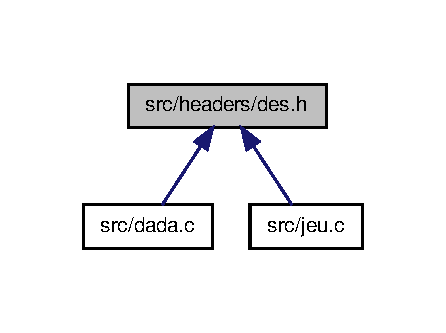
\includegraphics[width=214pt]{des_8h__dep__incl}
\end{center}
\end{figure}
\subsection*{Fonctions}
\begin{DoxyCompactItemize}
\item 
void \hyperlink{des_8h_af951d515465516d4056cec3f4571ee28}{init\-\_\-alea} ()
\begin{DoxyCompactList}\small\item\em Initialise le generateur de nombres aleatoires. \end{DoxyCompactList}\item 
int \hyperlink{des_8h_a2d90f82862986ff270f16f9771580b53}{lancer\-\_\-des} ()
\begin{DoxyCompactList}\small\item\em Simule un lancé de dé à 6 cotés. \end{DoxyCompactList}\end{DoxyCompactItemize}


\subsection{Description détaillée}
Declaration des fonctions relatives au des pour le jeu Petits chevaux. \begin{DoxyAuthor}{Auteur}
A\-O\-U\-N Abel et D\-O\-U\-C\-H\-E\-T Maximilien 
\end{DoxyAuthor}


Définition dans le fichier \hyperlink{des_8h_source}{des.\-h}.



\subsection{Documentation des fonctions}
\hypertarget{des_8h_af951d515465516d4056cec3f4571ee28}{\index{des.\-h@{des.\-h}!init\-\_\-alea@{init\-\_\-alea}}
\index{init\-\_\-alea@{init\-\_\-alea}!des.h@{des.\-h}}
\subsubsection[{init\-\_\-alea}]{\setlength{\rightskip}{0pt plus 5cm}void init\-\_\-alea (
\begin{DoxyParamCaption}
{}
\end{DoxyParamCaption}
)}}\label{des_8h_af951d515465516d4056cec3f4571ee28}


Initialise le generateur de nombres aleatoires. 

Initialise la graine allant servir pour la génération de nombres aléatoire. \begin{DoxyReturn}{Renvoie}
Void 
\end{DoxyReturn}


Définition à la ligne 16 du fichier des.\-c.



Voici le graphe des appelants de cette fonction \-:\nopagebreak
\begin{figure}[H]
\begin{center}
\leavevmode
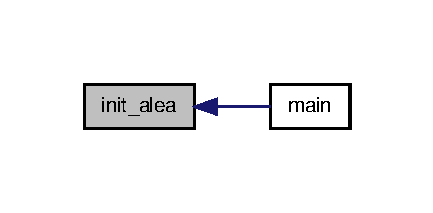
\includegraphics[width=208pt]{des_8h_af951d515465516d4056cec3f4571ee28_icgraph}
\end{center}
\end{figure}


\hypertarget{des_8h_a2d90f82862986ff270f16f9771580b53}{\index{des.\-h@{des.\-h}!lancer\-\_\-des@{lancer\-\_\-des}}
\index{lancer\-\_\-des@{lancer\-\_\-des}!des.h@{des.\-h}}
\subsubsection[{lancer\-\_\-des}]{\setlength{\rightskip}{0pt plus 5cm}int lancer\-\_\-des (
\begin{DoxyParamCaption}
{}
\end{DoxyParamCaption}
)}}\label{des_8h_a2d90f82862986ff270f16f9771580b53}


Simule un lancé de dé à 6 cotés. 

\begin{DoxyReturn}{Renvoie}
Int -\/ Compris entre 1 et 6. 
\end{DoxyReturn}


Définition à la ligne 25 du fichier des.\-c.



Voici le graphe des appelants de cette fonction \-:\nopagebreak
\begin{figure}[H]
\begin{center}
\leavevmode
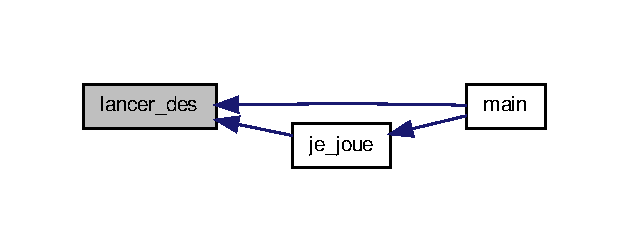
\includegraphics[width=302pt]{des_8h_a2d90f82862986ff270f16f9771580b53_icgraph}
\end{center}
\end{figure}



\hypertarget{jeu_8h}{\section{Référence du fichier src/headers/jeu.h}
\label{jeu_8h}\index{src/headers/jeu.\-h@{src/headers/jeu.\-h}}
}


Declaration des fonctions relatives au jeu pour le jeu Petits chevaux.  


Ce graphe montre quels fichiers incluent directement ou indirectement ce fichier \-:
\nopagebreak
\begin{figure}[H]
\begin{center}
\leavevmode
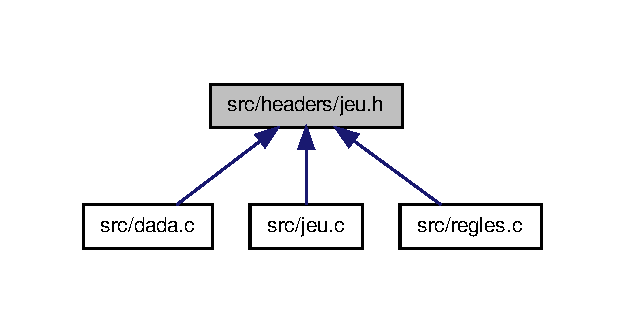
\includegraphics[width=300pt]{jeu_8h__dep__incl}
\end{center}
\end{figure}
\subsection*{Structures de données}
\begin{DoxyCompactItemize}
\item 
struct \hyperlink{structstruct__debuttour}{struct\-\_\-debuttour}
\begin{DoxyCompactList}\small\item\em Informations transmises par le pere pour les joueurs en debut de tour. \end{DoxyCompactList}\item 
struct \hyperlink{structstruct__retourjeu}{struct\-\_\-retourjeu}
\begin{DoxyCompactList}\small\item\em Informations transmises par les joueurs pour le pere en fin de tour. \end{DoxyCompactList}\item 
struct \hyperlink{structstruct__pendantjeu}{struct\-\_\-pendantjeu}
\begin{DoxyCompactList}\small\item\em Informations transmises par les joueurs pour les autres joueurs pendant le tour. \end{DoxyCompactList}\end{DoxyCompactItemize}
\subsection*{Définitions de type}
\begin{DoxyCompactItemize}
\item 
typedef struct \hyperlink{structstruct__debuttour}{struct\-\_\-debuttour} \hyperlink{jeu_8h_aa61fba51166ecbbbbe4ee5a1d0edde53}{struct\-\_\-debuttour}
\item 
typedef struct \hyperlink{structstruct__retourjeu}{struct\-\_\-retourjeu} \hyperlink{jeu_8h_ab10a026c12542d58ca83220094aec2b7}{struct\-\_\-retourjeu}
\item 
typedef struct \hyperlink{structstruct__pendantjeu}{struct\-\_\-pendantjeu} \hyperlink{jeu_8h_a85dbe6dd1eedca012ec9c4cf64adfb75}{struct\-\_\-pendantjeu}
\end{DoxyCompactItemize}
\subsection*{Fonctions}
\begin{DoxyCompactItemize}
\item 
int \hyperlink{jeu_8h_aad47be4fef9e94264139f82a73b259ae}{premier\-\_\-joueur} (void)
\begin{DoxyCompactList}\small\item\em Selection par l'utilisateur du premier joueur. \end{DoxyCompactList}\item 
void \hyperlink{jeu_8h_a725da0480654655d9b7fefa6c8b8ec1d}{cest\-\_\-a\-\_\-qui\-\_\-de\-\_\-jouer} (int num\-\_\-fils, int $\ast$$\ast$pipes, \hyperlink{structstruct__debuttour}{struct\-\_\-debuttour} $\ast$debuttourlu)
\begin{DoxyCompactList}\small\item\em Recupere les informations pour le prochain tour. \end{DoxyCompactList}\item 
int \hyperlink{jeu_8h_a9b781c5cf503cd1379cd5363baf5518b}{la\-\_\-partie\-\_\-est\-\_\-interrompue} (\hyperlink{structstruct__debuttour}{struct\-\_\-debuttour} $\ast$debuttourlu)
\begin{DoxyCompactList}\small\item\em Verifie si la partie n'a pas été interrompue. \end{DoxyCompactList}\item 
int \hyperlink{jeu_8h_a5775c2fd2b9eff5f551a8a923884583f}{je\-\_\-joue} (int num\-\_\-fils, int $\ast$position\-\_\-joueur, \hyperlink{structstruct__pendantjeu}{struct\-\_\-pendantjeu} $\ast$pendantjeu, int $\ast$danslescalier)
\begin{DoxyCompactList}\small\item\em Action effectuées par le joueur lorsque que vient son tour. \end{DoxyCompactList}\item 
void \hyperlink{jeu_8h_a0a25bcc79238a489f286585b395ccd17}{je\-\_\-transmet\-\_\-mon\-\_\-resultat\-\_\-au\-\_\-voisin} (int num\-\_\-fils, int $\ast$$\ast$pipes, \hyperlink{structstruct__pendantjeu}{struct\-\_\-pendantjeu} $\ast$pendantjeu)
\begin{DoxyCompactList}\small\item\em Transmission des informations du jeu d'un joueurs aux autres joueurs. \end{DoxyCompactList}\item 
void \hyperlink{jeu_8h_af71947ee506f911a3e0b09dd28198e5e}{jattend\-\_\-que\-\_\-linfo\-\_\-fasse\-\_\-le\-\_\-tour} (int num\-\_\-fils, int $\ast$$\ast$pipes, \hyperlink{structstruct__pendantjeu}{struct\-\_\-pendantjeu} $\ast$pendantjeulu)
\begin{DoxyCompactList}\small\item\em Attente après envoie des informations du retour de ces informations. \end{DoxyCompactList}\item 
void \hyperlink{jeu_8h_afbccfff41a7a1c5872f6f129a8a9ab44}{je\-\_\-fais\-\_\-passer\-\_\-le\-\_\-message} (int num\-\_\-fils, int $\ast$$\ast$pipes, \hyperlink{structstruct__pendantjeu}{struct\-\_\-pendantjeu} $\ast$pendantjeulu)
\begin{DoxyCompactList}\small\item\em Fait passer les informations au suivant. \end{DoxyCompactList}\item 
void \hyperlink{jeu_8h_aedc8c2b1001e2680710ac7ef3d73cac8}{je\-\_\-transmet\-\_\-mon\-\_\-resultat\-\_\-au\-\_\-pere} (int num\-\_\-fils, int $\ast$$\ast$pipes, \hyperlink{structstruct__retourjeu}{struct\-\_\-retourjeu} $\ast$retourjeu, int resultatde, int positionjoueur)
\begin{DoxyCompactList}\small\item\em Transmet les informations au père. \end{DoxyCompactList}\item 
void \hyperlink{jeu_8h_a2a267585992923972c7c142df69c5b89}{pere\-\_\-envoyer\-\_\-message\-\_\-aux\-\_\-fils} (int $\ast$$\ast$pipes, \hyperlink{structstruct__debuttour}{struct\-\_\-debuttour} $\ast$debuttour, int numerojoueur, int partieencours)
\begin{DoxyCompactList}\small\item\em Transmet les informations du père vers les fils. \end{DoxyCompactList}\item 
void \hyperlink{jeu_8h_a96da99031da1d74f38b559243dad2171}{pere\-\_\-lit\-\_\-retour\-\_\-tour} (int $\ast$$\ast$pipes, \hyperlink{structstruct__retourjeu}{struct\-\_\-retourjeu} $\ast$retourjeulu)
\begin{DoxyCompactList}\small\item\em Lecture des informations transmises par les fils. \end{DoxyCompactList}\item 
int \hyperlink{jeu_8h_ab99f683f90789787a7d8201407214cc1}{joueur\-\_\-suivant} (\hyperlink{structstruct__retourjeu}{struct\-\_\-retourjeu} $\ast$retourjeulu)
\begin{DoxyCompactList}\small\item\em Indique le prochain joueur devant jouer. \end{DoxyCompactList}\end{DoxyCompactItemize}


\subsection{Description détaillée}
Declaration des fonctions relatives au jeu pour le jeu Petits chevaux. \begin{DoxyAuthor}{Auteur}
A\-O\-U\-N Abel et D\-O\-U\-C\-H\-E\-T Maximilien 
\end{DoxyAuthor}


Définition dans le fichier \hyperlink{jeu_8h_source}{jeu.\-h}.



\subsection{Documentation des définitions de type}
\hypertarget{jeu_8h_aa61fba51166ecbbbbe4ee5a1d0edde53}{\index{jeu.\-h@{jeu.\-h}!struct\-\_\-debuttour@{struct\-\_\-debuttour}}
\index{struct\-\_\-debuttour@{struct\-\_\-debuttour}!jeu.h@{jeu.\-h}}
\subsubsection[{struct\-\_\-debuttour}]{\setlength{\rightskip}{0pt plus 5cm}typedef struct {\bf struct\-\_\-debuttour}  {\bf struct\-\_\-debuttour}}}\label{jeu_8h_aa61fba51166ecbbbbe4ee5a1d0edde53}
\hypertarget{jeu_8h_a85dbe6dd1eedca012ec9c4cf64adfb75}{\index{jeu.\-h@{jeu.\-h}!struct\-\_\-pendantjeu@{struct\-\_\-pendantjeu}}
\index{struct\-\_\-pendantjeu@{struct\-\_\-pendantjeu}!jeu.h@{jeu.\-h}}
\subsubsection[{struct\-\_\-pendantjeu}]{\setlength{\rightskip}{0pt plus 5cm}typedef struct {\bf struct\-\_\-pendantjeu}  {\bf struct\-\_\-pendantjeu}}}\label{jeu_8h_a85dbe6dd1eedca012ec9c4cf64adfb75}
\hypertarget{jeu_8h_ab10a026c12542d58ca83220094aec2b7}{\index{jeu.\-h@{jeu.\-h}!struct\-\_\-retourjeu@{struct\-\_\-retourjeu}}
\index{struct\-\_\-retourjeu@{struct\-\_\-retourjeu}!jeu.h@{jeu.\-h}}
\subsubsection[{struct\-\_\-retourjeu}]{\setlength{\rightskip}{0pt plus 5cm}typedef struct {\bf struct\-\_\-retourjeu}  {\bf struct\-\_\-retourjeu}}}\label{jeu_8h_ab10a026c12542d58ca83220094aec2b7}


\subsection{Documentation des fonctions}
\hypertarget{jeu_8h_a725da0480654655d9b7fefa6c8b8ec1d}{\index{jeu.\-h@{jeu.\-h}!cest\-\_\-a\-\_\-qui\-\_\-de\-\_\-jouer@{cest\-\_\-a\-\_\-qui\-\_\-de\-\_\-jouer}}
\index{cest\-\_\-a\-\_\-qui\-\_\-de\-\_\-jouer@{cest\-\_\-a\-\_\-qui\-\_\-de\-\_\-jouer}!jeu.h@{jeu.\-h}}
\subsubsection[{cest\-\_\-a\-\_\-qui\-\_\-de\-\_\-jouer}]{\setlength{\rightskip}{0pt plus 5cm}void cest\-\_\-a\-\_\-qui\-\_\-de\-\_\-jouer (
\begin{DoxyParamCaption}
\item[{int}]{num\-\_\-fils, }
\item[{int $\ast$$\ast$}]{pipes, }
\item[{{\bf struct\-\_\-debuttour} $\ast$}]{debuttourlu}
\end{DoxyParamCaption}
)}}\label{jeu_8h_a725da0480654655d9b7fefa6c8b8ec1d}


Recupere les informations pour le prochain tour. 

Récupère dans le pipe venant du main vers le joueur concerné la structure contenant les informations pour le prochain tour. 
\begin{DoxyParams}{Paramètres}
{\em num\-\_\-fils} & Int -\/ Correspond au numéro du fils souhaitant récupérer les informations. \\
\hline
{\em pipes} & Tableau des pipes. \\
\hline
{\em debuttourlu} & Pointeur sur la structure. \\
\hline
\end{DoxyParams}
\begin{DoxyReturn}{Renvoie}
Void 
\end{DoxyReturn}


Définition à la ligne 46 du fichier jeu.\-c.



Voici le graphe d'appel pour cette fonction \-:\nopagebreak
\begin{figure}[H]
\begin{center}
\leavevmode
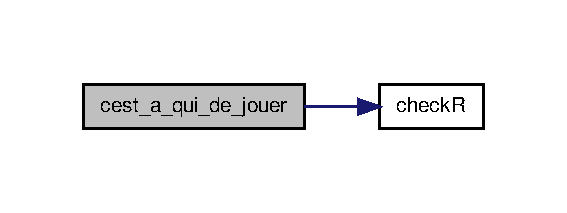
\includegraphics[width=272pt]{jeu_8h_a725da0480654655d9b7fefa6c8b8ec1d_cgraph}
\end{center}
\end{figure}




Voici le graphe des appelants de cette fonction \-:\nopagebreak
\begin{figure}[H]
\begin{center}
\leavevmode
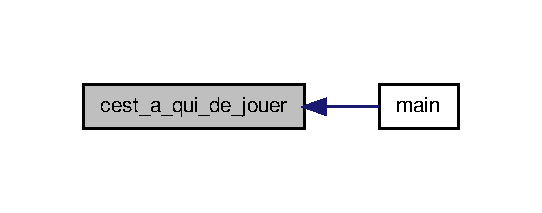
\includegraphics[width=260pt]{jeu_8h_a725da0480654655d9b7fefa6c8b8ec1d_icgraph}
\end{center}
\end{figure}


\hypertarget{jeu_8h_af71947ee506f911a3e0b09dd28198e5e}{\index{jeu.\-h@{jeu.\-h}!jattend\-\_\-que\-\_\-linfo\-\_\-fasse\-\_\-le\-\_\-tour@{jattend\-\_\-que\-\_\-linfo\-\_\-fasse\-\_\-le\-\_\-tour}}
\index{jattend\-\_\-que\-\_\-linfo\-\_\-fasse\-\_\-le\-\_\-tour@{jattend\-\_\-que\-\_\-linfo\-\_\-fasse\-\_\-le\-\_\-tour}!jeu.h@{jeu.\-h}}
\subsubsection[{jattend\-\_\-que\-\_\-linfo\-\_\-fasse\-\_\-le\-\_\-tour}]{\setlength{\rightskip}{0pt plus 5cm}void jattend\-\_\-que\-\_\-linfo\-\_\-fasse\-\_\-le\-\_\-tour (
\begin{DoxyParamCaption}
\item[{int}]{num\-\_\-fils, }
\item[{int $\ast$$\ast$}]{pipes, }
\item[{{\bf struct\-\_\-pendantjeu} $\ast$}]{pendantjeulu}
\end{DoxyParamCaption}
)}}\label{jeu_8h_af71947ee506f911a3e0b09dd28198e5e}


Attente après envoie des informations du retour de ces informations. 

Permet la récupération des informations envoyés par le biais du joueur précédent. Ce en lisant dans le pipe du joueur précédent le num\-\_\-fils. Quand l'information sera revenue, elle aura fait le tour. 
\begin{DoxyParams}{Paramètres}
{\em num\-\_\-fils} & Int -\/ Correspond au numéro du fils souhaitant récupérer les informations. \\
\hline
{\em pipes} & Tableau des pipes. \\
\hline
{\em pendantjeulu} & Pointeur sur la structure contenant les informations du jeu qui vient d'être fait et transmis par le voisin précédent. \\
\hline
\end{DoxyParams}
\begin{DoxyReturn}{Renvoie}
Void -\/ Termine en cas d'erreur 
\end{DoxyReturn}


Définition à la ligne 107 du fichier jeu.\-c.



Voici le graphe d'appel pour cette fonction \-:\nopagebreak
\begin{figure}[H]
\begin{center}
\leavevmode
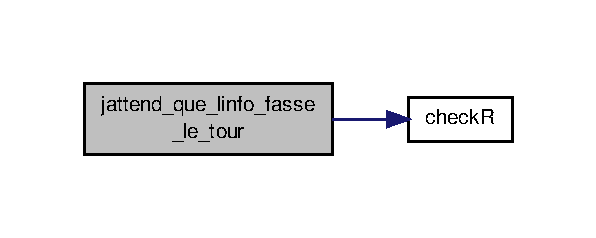
\includegraphics[width=286pt]{jeu_8h_af71947ee506f911a3e0b09dd28198e5e_cgraph}
\end{center}
\end{figure}




Voici le graphe des appelants de cette fonction \-:\nopagebreak
\begin{figure}[H]
\begin{center}
\leavevmode
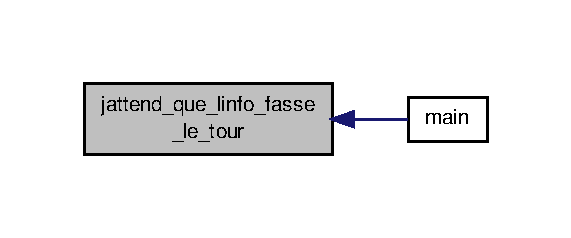
\includegraphics[width=274pt]{jeu_8h_af71947ee506f911a3e0b09dd28198e5e_icgraph}
\end{center}
\end{figure}


\hypertarget{jeu_8h_afbccfff41a7a1c5872f6f129a8a9ab44}{\index{jeu.\-h@{jeu.\-h}!je\-\_\-fais\-\_\-passer\-\_\-le\-\_\-message@{je\-\_\-fais\-\_\-passer\-\_\-le\-\_\-message}}
\index{je\-\_\-fais\-\_\-passer\-\_\-le\-\_\-message@{je\-\_\-fais\-\_\-passer\-\_\-le\-\_\-message}!jeu.h@{jeu.\-h}}
\subsubsection[{je\-\_\-fais\-\_\-passer\-\_\-le\-\_\-message}]{\setlength{\rightskip}{0pt plus 5cm}void je\-\_\-fais\-\_\-passer\-\_\-le\-\_\-message (
\begin{DoxyParamCaption}
\item[{int}]{num\-\_\-fils, }
\item[{int $\ast$$\ast$}]{pipes, }
\item[{{\bf struct\-\_\-pendantjeu} $\ast$}]{pendantjeulu}
\end{DoxyParamCaption}
)}}\label{jeu_8h_afbccfff41a7a1c5872f6f129a8a9ab44}


Fait passer les informations au suivant. 

Permet la transmission des informations envoyés par le biais du joueur précédent. Ce en lisant dans le pipe du joueur précédent le num\-\_\-fils. On l'envoie au suivant immédiatement. Cela nous permet d'appliquer la regle pour que le joueur revienne au point de départ si un autre joueur est arrivé sur la même case. Cette fonction est appellée lorsque ce n'est pas à num\-\_\-fils de jouer. 
\begin{DoxyParams}{Paramètres}
{\em num\-\_\-fils} & Int -\/ Correspond au numéro du fils souhaitant récupérer les informations. \\
\hline
{\em pipes} & Tableau des pipes. \\
\hline
{\em pendantjeulu} & Pointeur sur la structure contenant les informations du jeu qui vient d'être transmis par le voisin précédent. \\
\hline
\end{DoxyParams}
\begin{DoxyReturn}{Renvoie}
Void -\/ Termine en cas d'erreur 
\end{DoxyReturn}


Définition à la ligne 128 du fichier jeu.\-c.



Voici le graphe d'appel pour cette fonction \-:\nopagebreak
\begin{figure}[H]
\begin{center}
\leavevmode
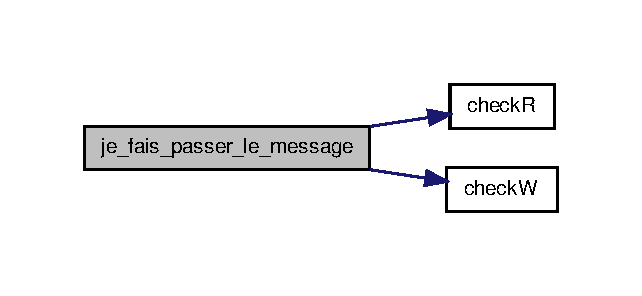
\includegraphics[width=308pt]{jeu_8h_afbccfff41a7a1c5872f6f129a8a9ab44_cgraph}
\end{center}
\end{figure}




Voici le graphe des appelants de cette fonction \-:\nopagebreak
\begin{figure}[H]
\begin{center}
\leavevmode
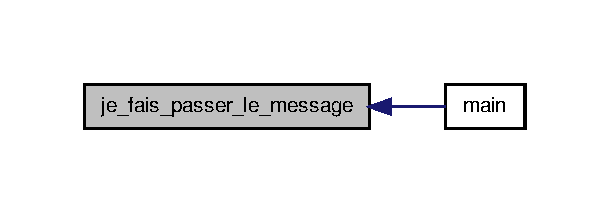
\includegraphics[width=292pt]{jeu_8h_afbccfff41a7a1c5872f6f129a8a9ab44_icgraph}
\end{center}
\end{figure}


\hypertarget{jeu_8h_a5775c2fd2b9eff5f551a8a923884583f}{\index{jeu.\-h@{jeu.\-h}!je\-\_\-joue@{je\-\_\-joue}}
\index{je\-\_\-joue@{je\-\_\-joue}!jeu.h@{jeu.\-h}}
\subsubsection[{je\-\_\-joue}]{\setlength{\rightskip}{0pt plus 5cm}int je\-\_\-joue (
\begin{DoxyParamCaption}
\item[{int}]{num\-\_\-fils, }
\item[{int $\ast$}]{positionjoueur, }
\item[{{\bf struct\-\_\-pendantjeu} $\ast$}]{pendantjeu, }
\item[{int $\ast$}]{danslescalier}
\end{DoxyParamCaption}
)}}\label{jeu_8h_a5775c2fd2b9eff5f551a8a923884583f}


Action effectuées par le joueur lorsque que vient son tour. 

Le joueur lance un dé, demande aux reglès quelle est sa nouvelle position et enregistre ces informations. 
\begin{DoxyParams}{Paramètres}
{\em num\-\_\-fils} & Int -\/ Correspond au numéro du fils souhaitant récupérer les informations. \\
\hline
{\em positionjoueur} & Pointeur sur la position du joueur appelant la fonction. \\
\hline
{\em pendantjeu} & Pointeur sur la structure qui va être transmise aux autres joueurs. \\
\hline
\end{DoxyParams}
\begin{DoxyReturn}{Renvoie}
Int -\/ Retourne le resultat du lancé de dé, la position est déjà modifiée. 
\end{DoxyReturn}


Définition à la ligne 71 du fichier jeu.\-c.



Voici le graphe d'appel pour cette fonction \-:\nopagebreak
\begin{figure}[H]
\begin{center}
\leavevmode
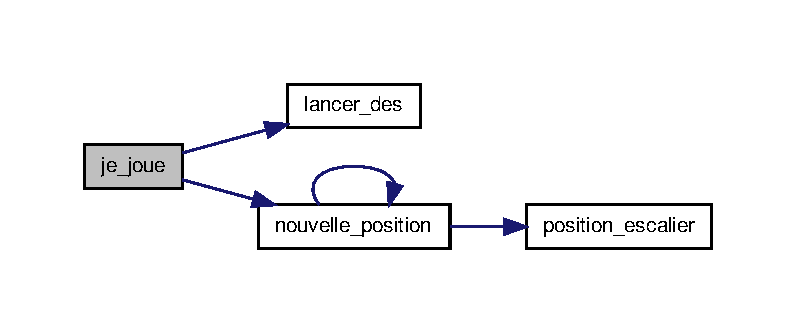
\includegraphics[width=350pt]{jeu_8h_a5775c2fd2b9eff5f551a8a923884583f_cgraph}
\end{center}
\end{figure}




Voici le graphe des appelants de cette fonction \-:\nopagebreak
\begin{figure}[H]
\begin{center}
\leavevmode
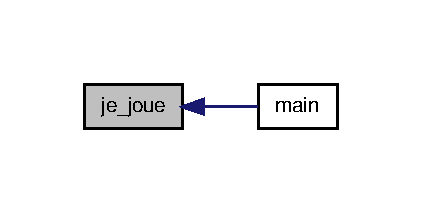
\includegraphics[width=202pt]{jeu_8h_a5775c2fd2b9eff5f551a8a923884583f_icgraph}
\end{center}
\end{figure}


\hypertarget{jeu_8h_aedc8c2b1001e2680710ac7ef3d73cac8}{\index{jeu.\-h@{jeu.\-h}!je\-\_\-transmet\-\_\-mon\-\_\-resultat\-\_\-au\-\_\-pere@{je\-\_\-transmet\-\_\-mon\-\_\-resultat\-\_\-au\-\_\-pere}}
\index{je\-\_\-transmet\-\_\-mon\-\_\-resultat\-\_\-au\-\_\-pere@{je\-\_\-transmet\-\_\-mon\-\_\-resultat\-\_\-au\-\_\-pere}!jeu.h@{jeu.\-h}}
\subsubsection[{je\-\_\-transmet\-\_\-mon\-\_\-resultat\-\_\-au\-\_\-pere}]{\setlength{\rightskip}{0pt plus 5cm}void je\-\_\-transmet\-\_\-mon\-\_\-resultat\-\_\-au\-\_\-pere (
\begin{DoxyParamCaption}
\item[{int}]{num\-\_\-fils, }
\item[{int $\ast$$\ast$}]{pipes, }
\item[{{\bf struct\-\_\-retourjeu} $\ast$}]{retourjeu, }
\item[{int}]{resultatde, }
\item[{int}]{positionjoueur}
\end{DoxyParamCaption}
)}}\label{jeu_8h_aedc8c2b1001e2680710ac7ef3d73cac8}


Transmet les informations au père. 

Quand les informations transmises ont fait le tour, on génère une structure contenant les informations dont le père aura besoin pour modérer. On lui envoie alors dans le pipe des fils vers le père. 
\begin{DoxyParams}{Paramètres}
{\em num\-\_\-fils} & Int -\/ Correspond au numéro du fils souhaitant récupérer les informations. \\
\hline
{\em pipes} & Tableau des pipes. \\
\hline
{\em retourjeu} & Pointeur sur la structure contenant les informations du jeu qui vient d'être fait et ayant fait le tour. \\
\hline
{\em resultatde} & Valeur du dé lancé. Utile pour le père afin de savoir si le fils doit rejouer ou non. En cas de double 6. \\
\hline
{\em positionjoueur} & Nouvelle position du joueur. Utile pour savoir si un joueur est arrivé au bout de sa course. \\
\hline
\end{DoxyParams}
\begin{DoxyReturn}{Renvoie}
Void -\/ Termine en cas d'erreur 
\end{DoxyReturn}


Définition à la ligne 157 du fichier jeu.\-c.



Voici le graphe d'appel pour cette fonction \-:\nopagebreak
\begin{figure}[H]
\begin{center}
\leavevmode
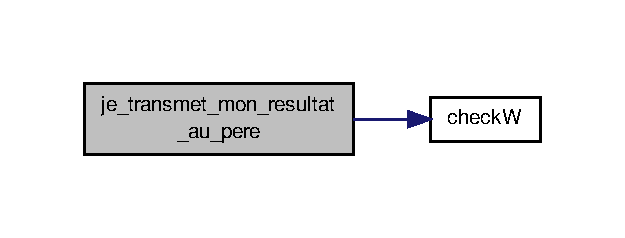
\includegraphics[width=300pt]{jeu_8h_aedc8c2b1001e2680710ac7ef3d73cac8_cgraph}
\end{center}
\end{figure}




Voici le graphe des appelants de cette fonction \-:\nopagebreak
\begin{figure}[H]
\begin{center}
\leavevmode
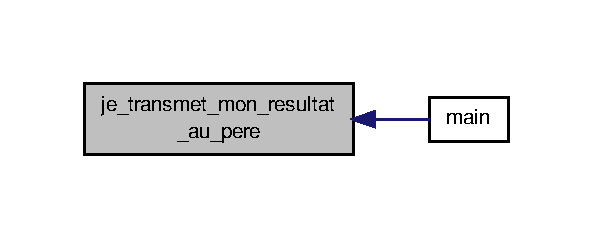
\includegraphics[width=284pt]{jeu_8h_aedc8c2b1001e2680710ac7ef3d73cac8_icgraph}
\end{center}
\end{figure}


\hypertarget{jeu_8h_a0a25bcc79238a489f286585b395ccd17}{\index{jeu.\-h@{jeu.\-h}!je\-\_\-transmet\-\_\-mon\-\_\-resultat\-\_\-au\-\_\-voisin@{je\-\_\-transmet\-\_\-mon\-\_\-resultat\-\_\-au\-\_\-voisin}}
\index{je\-\_\-transmet\-\_\-mon\-\_\-resultat\-\_\-au\-\_\-voisin@{je\-\_\-transmet\-\_\-mon\-\_\-resultat\-\_\-au\-\_\-voisin}!jeu.h@{jeu.\-h}}
\subsubsection[{je\-\_\-transmet\-\_\-mon\-\_\-resultat\-\_\-au\-\_\-voisin}]{\setlength{\rightskip}{0pt plus 5cm}void je\-\_\-transmet\-\_\-mon\-\_\-resultat\-\_\-au\-\_\-voisin (
\begin{DoxyParamCaption}
\item[{int}]{num\-\_\-fils, }
\item[{int $\ast$$\ast$}]{pipes, }
\item[{{\bf struct\-\_\-pendantjeu} $\ast$}]{pendantjeu}
\end{DoxyParamCaption}
)}}\label{jeu_8h_a0a25bcc79238a489f286585b395ccd17}


Transmission des informations du jeu d'un joueurs aux autres joueurs. 

La structure contenant les informations du jeu qui vient d'être effectué est déjà crée. Il ne reste qu'a l'écrire dans le pipe du voisin. 
\begin{DoxyParams}{Paramètres}
{\em num\-\_\-fils} & Int -\/ Correspond au numéro du fils souhaitant récupérer les informations. \\
\hline
{\em pipes} & Tableau des pipes. \\
\hline
{\em pendantjeu} & Pointeur sur la structure contenant les informations du jeu qui vient d'être fait. \\
\hline
\end{DoxyParams}
\begin{DoxyReturn}{Renvoie}
Void -\/ Termine en cas d'erreur 
\end{DoxyReturn}


Définition à la ligne 92 du fichier jeu.\-c.



Voici le graphe d'appel pour cette fonction \-:\nopagebreak
\begin{figure}[H]
\begin{center}
\leavevmode
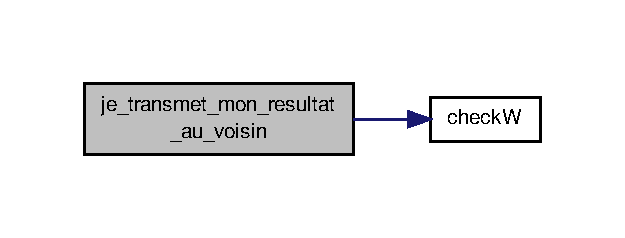
\includegraphics[width=300pt]{jeu_8h_a0a25bcc79238a489f286585b395ccd17_cgraph}
\end{center}
\end{figure}




Voici le graphe des appelants de cette fonction \-:\nopagebreak
\begin{figure}[H]
\begin{center}
\leavevmode
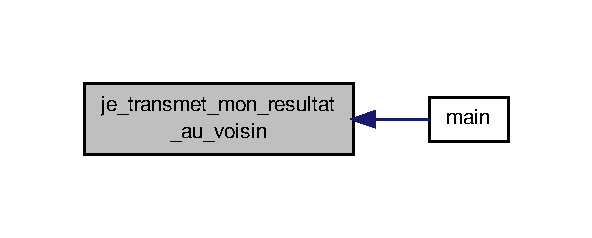
\includegraphics[width=284pt]{jeu_8h_a0a25bcc79238a489f286585b395ccd17_icgraph}
\end{center}
\end{figure}


\hypertarget{jeu_8h_ab99f683f90789787a7d8201407214cc1}{\index{jeu.\-h@{jeu.\-h}!joueur\-\_\-suivant@{joueur\-\_\-suivant}}
\index{joueur\-\_\-suivant@{joueur\-\_\-suivant}!jeu.h@{jeu.\-h}}
\subsubsection[{joueur\-\_\-suivant}]{\setlength{\rightskip}{0pt plus 5cm}int joueur\-\_\-suivant (
\begin{DoxyParamCaption}
\item[{{\bf struct\-\_\-retourjeu} $\ast$}]{retourjeulu}
\end{DoxyParamCaption}
)}}\label{jeu_8h_ab99f683f90789787a7d8201407214cc1}


Indique le prochain joueur devant jouer. 

Selon le retour des informations renvoyées au père après un tour de jeu. Le père décide si il fait rejouer un joueur (en cas de double 6), ou si il donne la main au suivant. 
\begin{DoxyParams}{Paramètres}
{\em retourjeulu} & Pointeur sur la structure devant contenir les informations destinées au père par le joueurs. \\
\hline
\end{DoxyParams}
\begin{DoxyReturn}{Renvoie}
result Int -\/ Le numéro du prochain joueur devant s'executer. 
\end{DoxyReturn}


Définition à la ligne 207 du fichier jeu.\-c.



Voici le graphe des appelants de cette fonction \-:\nopagebreak
\begin{figure}[H]
\begin{center}
\leavevmode
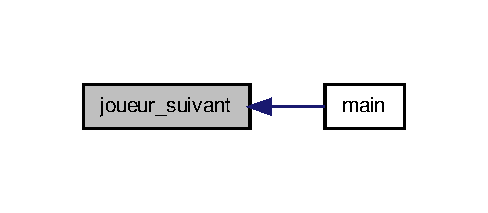
\includegraphics[width=234pt]{jeu_8h_ab99f683f90789787a7d8201407214cc1_icgraph}
\end{center}
\end{figure}


\hypertarget{jeu_8h_a9b781c5cf503cd1379cd5363baf5518b}{\index{jeu.\-h@{jeu.\-h}!la\-\_\-partie\-\_\-est\-\_\-interrompue@{la\-\_\-partie\-\_\-est\-\_\-interrompue}}
\index{la\-\_\-partie\-\_\-est\-\_\-interrompue@{la\-\_\-partie\-\_\-est\-\_\-interrompue}!jeu.h@{jeu.\-h}}
\subsubsection[{la\-\_\-partie\-\_\-est\-\_\-interrompue}]{\setlength{\rightskip}{0pt plus 5cm}int la\-\_\-partie\-\_\-est\-\_\-interrompue (
\begin{DoxyParamCaption}
\item[{{\bf struct\-\_\-debuttour} $\ast$}]{debuttourlu}
\end{DoxyParamCaption}
)}}\label{jeu_8h_a9b781c5cf503cd1379cd5363baf5518b}


Verifie si la partie n'a pas été interrompue. 

Dans le cas ou un joueur a gagné, nous considérons que la partie est finie. Dans le cas ou l'utilisateur choisi d'interrompre le programme cette fonction sera très utile pour permettre aux joueurs de se tuer même si ils n'ont pas fini de jouer. 
\begin{DoxyParams}{Paramètres}
{\em debuttourlu} & Pointeur sur la structure lue au debut du tour. \\
\hline
\end{DoxyParams}
\begin{DoxyReturn}{Renvoie}
Int -\/ Renvoie 1 si la partie est termine ou interrompue, 0 sinon. 
\end{DoxyReturn}


Définition à la ligne 58 du fichier jeu.\-c.



Voici le graphe des appelants de cette fonction \-:\nopagebreak
\begin{figure}[H]
\begin{center}
\leavevmode
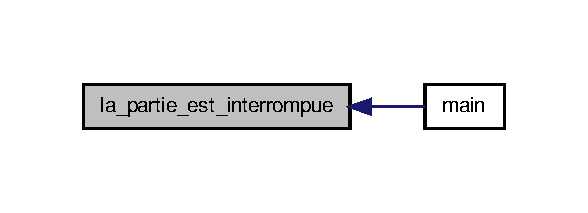
\includegraphics[width=282pt]{jeu_8h_a9b781c5cf503cd1379cd5363baf5518b_icgraph}
\end{center}
\end{figure}


\hypertarget{jeu_8h_a2a267585992923972c7c142df69c5b89}{\index{jeu.\-h@{jeu.\-h}!pere\-\_\-envoyer\-\_\-message\-\_\-aux\-\_\-fils@{pere\-\_\-envoyer\-\_\-message\-\_\-aux\-\_\-fils}}
\index{pere\-\_\-envoyer\-\_\-message\-\_\-aux\-\_\-fils@{pere\-\_\-envoyer\-\_\-message\-\_\-aux\-\_\-fils}!jeu.h@{jeu.\-h}}
\subsubsection[{pere\-\_\-envoyer\-\_\-message\-\_\-aux\-\_\-fils}]{\setlength{\rightskip}{0pt plus 5cm}void pere\-\_\-envoyer\-\_\-message\-\_\-aux\-\_\-fils (
\begin{DoxyParamCaption}
\item[{int $\ast$$\ast$}]{pipes, }
\item[{{\bf struct\-\_\-debuttour} $\ast$}]{debuttour, }
\item[{int}]{numerojoueur, }
\item[{int}]{partieencours}
\end{DoxyParamCaption}
)}}\label{jeu_8h_a2a267585992923972c7c142df69c5b89}


Transmet les informations du père vers les fils. 

Quand les informations transmises au père ont été analysé, ou lors du premier tour le père doit envoyer des informations au fils. 
\begin{DoxyParams}{Paramètres}
{\em pipes} & Tableau des pipes. \\
\hline
{\em debuttour} & Pointeur sur la structure devant contenir les informations qui vont être transmises au joueur. \\
\hline
{\em numerojoueur} & Numéro du prochain joueur devant jouer. \\
\hline
{\em partieencours} & Indique si la partie est toujours en cours. (1 oui $|$ 0 -\/ non) \\
\hline
\end{DoxyParams}
\begin{DoxyReturn}{Renvoie}
Void -\/ Termine en cas d'erreur 
\end{DoxyReturn}


Définition à la ligne 176 du fichier jeu.\-c.



Voici le graphe d'appel pour cette fonction \-:\nopagebreak
\begin{figure}[H]
\begin{center}
\leavevmode
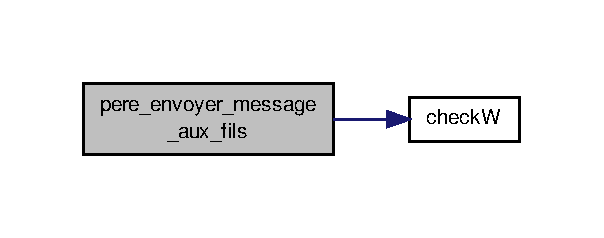
\includegraphics[width=290pt]{jeu_8h_a2a267585992923972c7c142df69c5b89_cgraph}
\end{center}
\end{figure}




Voici le graphe des appelants de cette fonction \-:\nopagebreak
\begin{figure}[H]
\begin{center}
\leavevmode
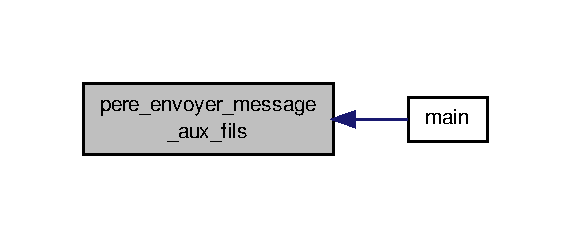
\includegraphics[width=274pt]{jeu_8h_a2a267585992923972c7c142df69c5b89_icgraph}
\end{center}
\end{figure}


\hypertarget{jeu_8h_a96da99031da1d74f38b559243dad2171}{\index{jeu.\-h@{jeu.\-h}!pere\-\_\-lit\-\_\-retour\-\_\-tour@{pere\-\_\-lit\-\_\-retour\-\_\-tour}}
\index{pere\-\_\-lit\-\_\-retour\-\_\-tour@{pere\-\_\-lit\-\_\-retour\-\_\-tour}!jeu.h@{jeu.\-h}}
\subsubsection[{pere\-\_\-lit\-\_\-retour\-\_\-tour}]{\setlength{\rightskip}{0pt plus 5cm}void pere\-\_\-lit\-\_\-retour\-\_\-tour (
\begin{DoxyParamCaption}
\item[{int $\ast$$\ast$}]{pipes, }
\item[{{\bf struct\-\_\-retourjeu} $\ast$}]{retourjeulu}
\end{DoxyParamCaption}
)}}\label{jeu_8h_a96da99031da1d74f38b559243dad2171}


Lecture des informations transmises par les fils. 

Le joueur qui vient de jouer fait remonter des informations au père une fois qu'il vient de terminer de faire circuler des informations aux autres joueurs. 
\begin{DoxyParams}{Paramètres}
{\em pipes} & Tableau des pipes. \\
\hline
{\em retourjeulu} & Pointeur sur la structure devant contenir les informations destinées au père par le joueurs. \\
\hline
\end{DoxyParams}
\begin{DoxyReturn}{Renvoie}
Void -\/ Termine en cas d'erreur 
\end{DoxyReturn}


Définition à la ligne 194 du fichier jeu.\-c.



Voici le graphe d'appel pour cette fonction \-:\nopagebreak
\begin{figure}[H]
\begin{center}
\leavevmode
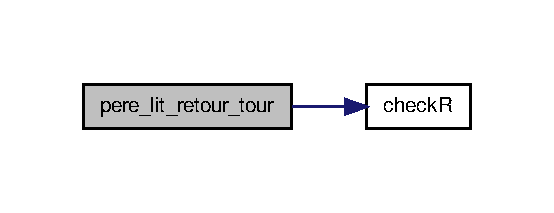
\includegraphics[width=266pt]{jeu_8h_a96da99031da1d74f38b559243dad2171_cgraph}
\end{center}
\end{figure}




Voici le graphe des appelants de cette fonction \-:\nopagebreak
\begin{figure}[H]
\begin{center}
\leavevmode
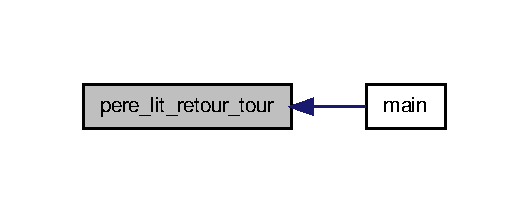
\includegraphics[width=254pt]{jeu_8h_a96da99031da1d74f38b559243dad2171_icgraph}
\end{center}
\end{figure}


\hypertarget{jeu_8h_aad47be4fef9e94264139f82a73b259ae}{\index{jeu.\-h@{jeu.\-h}!premier\-\_\-joueur@{premier\-\_\-joueur}}
\index{premier\-\_\-joueur@{premier\-\_\-joueur}!jeu.h@{jeu.\-h}}
\subsubsection[{premier\-\_\-joueur}]{\setlength{\rightskip}{0pt plus 5cm}int premier\-\_\-joueur (
\begin{DoxyParamCaption}
\item[{void}]{}
\end{DoxyParamCaption}
)}}\label{jeu_8h_aad47be4fef9e94264139f82a73b259ae}


Selection par l'utilisateur du premier joueur. 

Demande a l'utilisateur de saisir le numero du premier joueur. \begin{DoxyReturn}{Renvoie}
Int -\/ Retourne le numero du joueur saisi. 
\end{DoxyReturn}


Définition à la ligne 22 du fichier jeu.\-c.



Voici le graphe des appelants de cette fonction \-:\nopagebreak
\begin{figure}[H]
\begin{center}
\leavevmode
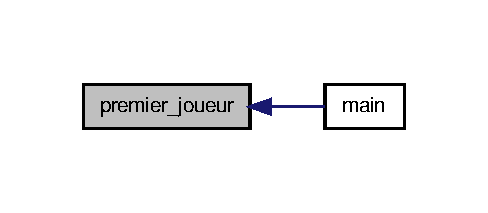
\includegraphics[width=234pt]{jeu_8h_aad47be4fef9e94264139f82a73b259ae_icgraph}
\end{center}
\end{figure}



\hypertarget{pipes_8h}{\section{Référence du fichier src/headers/pipes.h}
\label{pipes_8h}\index{src/headers/pipes.\-h@{src/headers/pipes.\-h}}
}


Declaration des fonctions relatives au pipes pour le jeu Petits chevaux.  


Ce graphe montre quels fichiers incluent directement ou indirectement ce fichier \-:
\nopagebreak
\begin{figure}[H]
\begin{center}
\leavevmode
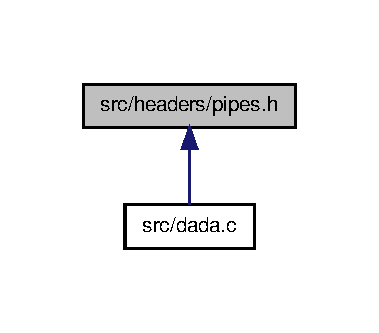
\includegraphics[width=182pt]{pipes_8h__dep__incl}
\end{center}
\end{figure}
\subsection*{Fonctions}
\begin{DoxyCompactItemize}
\item 
int \hyperlink{pipes_8h_a8efe620a19ac0e4f120345e57b6edeac}{creation\-\_\-pipes} (int $\ast$$\ast$pipes)
\begin{DoxyCompactList}\small\item\em Creation des pipes. \end{DoxyCompactList}\item 
int \hyperlink{pipes_8h_a4352c1ccc165cf89b0c4d6a748b1dd58}{pipes\-\_\-fils\-\_\-start\-\_\-close} (int num\-\_\-fils, int $\ast$$\ast$pipes)
\begin{DoxyCompactList}\small\item\em Fermeture des pipes non utilises pour chaque fils. \end{DoxyCompactList}\item 
int \hyperlink{pipes_8h_a07068e6f96cddd3caeaa6dde747270e7}{pipes\-\_\-fils\-\_\-end\-\_\-close} (int num\-\_\-fils, int $\ast$$\ast$pipes)
\begin{DoxyCompactList}\small\item\em Fermeture des pipes utilisés pour chaque fils. \end{DoxyCompactList}\item 
int \hyperlink{pipes_8h_a7e56d9b0553fa826c8087ce2d06d987d}{pipes\-\_\-pere\-\_\-start\-\_\-close} (int $\ast$$\ast$pipes)
\begin{DoxyCompactList}\small\item\em Fermeture des pipes non utilises pour le pere. \end{DoxyCompactList}\item 
int \hyperlink{pipes_8h_a66dbda032de023003f32d4f4eec66875}{pipes\-\_\-pere\-\_\-end\-\_\-close} (int $\ast$$\ast$pipes)
\begin{DoxyCompactList}\small\item\em Fermeture des pipes utilisés pour le père. \end{DoxyCompactList}\end{DoxyCompactItemize}


\subsection{Description détaillée}
Declaration des fonctions relatives au pipes pour le jeu Petits chevaux. \begin{DoxyAuthor}{Auteur}
A\-O\-U\-N Abel et D\-O\-U\-C\-H\-E\-T Maximilien
\end{DoxyAuthor}
Les pipes sont organisés de cette maniere \-: 0 -\/$>$ Entree du main depuis joueurs 1 -\/$>$ sortie du main vers joueur 1 2 -\/$>$ sortie du main vers joueur 2 3 -\/$>$ sortie du main vers joueur 3 4 -\/$>$ sortie du main vers joueur 4 5 -\/$>$ sortie du joueur 1 vers joueur 2 6 -\/$>$ sortie du joueur 2 vers joueur 3 7 -\/$>$ sortie du joueur 3 vers joueur 4 8 -\/$>$ sortie du joueur 4 vers joueur 1 

Définition dans le fichier \hyperlink{pipes_8h_source}{pipes.\-h}.



\subsection{Documentation des fonctions}
\hypertarget{pipes_8h_a8efe620a19ac0e4f120345e57b6edeac}{\index{pipes.\-h@{pipes.\-h}!creation\-\_\-pipes@{creation\-\_\-pipes}}
\index{creation\-\_\-pipes@{creation\-\_\-pipes}!pipes.h@{pipes.\-h}}
\subsubsection[{creation\-\_\-pipes}]{\setlength{\rightskip}{0pt plus 5cm}int creation\-\_\-pipes (
\begin{DoxyParamCaption}
\item[{int $\ast$$\ast$}]{pipes}
\end{DoxyParamCaption}
)}}\label{pipes_8h_a8efe620a19ac0e4f120345e57b6edeac}


Creation des pipes. 

Fonction de creation des pipes 
\begin{DoxyParams}{Paramètres}
{\em pipes} & Tableau des pipes \\
\hline
\end{DoxyParams}
\begin{DoxyReturn}{Renvoie}
Retourne 0 si tout s'est bien passé 
\end{DoxyReturn}


Définition à la ligne 28 du fichier pipes.\-c.



Voici le graphe des appelants de cette fonction \-:\nopagebreak
\begin{figure}[H]
\begin{center}
\leavevmode
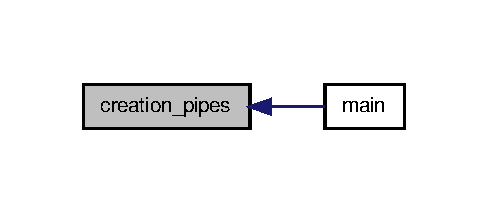
\includegraphics[width=234pt]{pipes_8h_a8efe620a19ac0e4f120345e57b6edeac_icgraph}
\end{center}
\end{figure}


\hypertarget{pipes_8h_a07068e6f96cddd3caeaa6dde747270e7}{\index{pipes.\-h@{pipes.\-h}!pipes\-\_\-fils\-\_\-end\-\_\-close@{pipes\-\_\-fils\-\_\-end\-\_\-close}}
\index{pipes\-\_\-fils\-\_\-end\-\_\-close@{pipes\-\_\-fils\-\_\-end\-\_\-close}!pipes.h@{pipes.\-h}}
\subsubsection[{pipes\-\_\-fils\-\_\-end\-\_\-close}]{\setlength{\rightskip}{0pt plus 5cm}int pipes\-\_\-fils\-\_\-end\-\_\-close (
\begin{DoxyParamCaption}
\item[{int}]{num\-\_\-fils, }
\item[{int $\ast$$\ast$}]{pipes}
\end{DoxyParamCaption}
)}}\label{pipes_8h_a07068e6f96cddd3caeaa6dde747270e7}


Fermeture des pipes utilisés pour chaque fils. 

Ferme les pipes de chaque fils utilisés lorsque qu'il n'en a plus besoin. 
\begin{DoxyParams}{Paramètres}
{\em num\-\_\-fils} & Le numéro du fils souhaitant fermer ses pipes \\
\hline
{\em pipes} & Le Tableau des pipes \\
\hline
\end{DoxyParams}
\begin{DoxyReturn}{Renvoie}
Retourne 0 si tout s'est bien passé 
\end{DoxyReturn}


Définition à la ligne 82 du fichier pipes.\-c.



Voici le graphe des appelants de cette fonction \-:\nopagebreak
\begin{figure}[H]
\begin{center}
\leavevmode
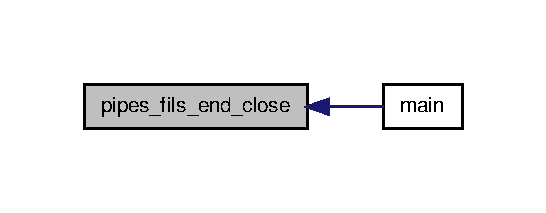
\includegraphics[width=262pt]{pipes_8h_a07068e6f96cddd3caeaa6dde747270e7_icgraph}
\end{center}
\end{figure}


\hypertarget{pipes_8h_a4352c1ccc165cf89b0c4d6a748b1dd58}{\index{pipes.\-h@{pipes.\-h}!pipes\-\_\-fils\-\_\-start\-\_\-close@{pipes\-\_\-fils\-\_\-start\-\_\-close}}
\index{pipes\-\_\-fils\-\_\-start\-\_\-close@{pipes\-\_\-fils\-\_\-start\-\_\-close}!pipes.h@{pipes.\-h}}
\subsubsection[{pipes\-\_\-fils\-\_\-start\-\_\-close}]{\setlength{\rightskip}{0pt plus 5cm}int pipes\-\_\-fils\-\_\-start\-\_\-close (
\begin{DoxyParamCaption}
\item[{int}]{num\-\_\-fils, }
\item[{int $\ast$$\ast$}]{pipes}
\end{DoxyParamCaption}
)}}\label{pipes_8h_a4352c1ccc165cf89b0c4d6a748b1dd58}


Fermeture des pipes non utilises pour chaque fils. 

Ferme les pipes de chaque fils non utilisés. 
\begin{DoxyParams}{Paramètres}
{\em num\-\_\-fils} & Le numéro du fils souhaitant fermer ses pipes \\
\hline
{\em pipes} & Le Tableau des pipes \\
\hline
\end{DoxyParams}
\begin{DoxyReturn}{Renvoie}
Retourne 0 si tout s'est bien passé 
\end{DoxyReturn}


Définition à la ligne 47 du fichier pipes.\-c.



Voici le graphe des appelants de cette fonction \-:\nopagebreak
\begin{figure}[H]
\begin{center}
\leavevmode
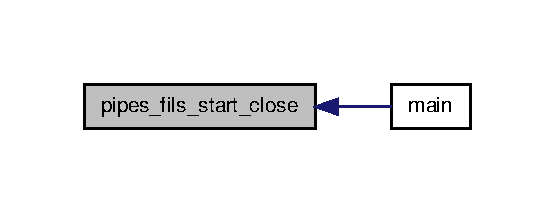
\includegraphics[width=266pt]{pipes_8h_a4352c1ccc165cf89b0c4d6a748b1dd58_icgraph}
\end{center}
\end{figure}


\hypertarget{pipes_8h_a66dbda032de023003f32d4f4eec66875}{\index{pipes.\-h@{pipes.\-h}!pipes\-\_\-pere\-\_\-end\-\_\-close@{pipes\-\_\-pere\-\_\-end\-\_\-close}}
\index{pipes\-\_\-pere\-\_\-end\-\_\-close@{pipes\-\_\-pere\-\_\-end\-\_\-close}!pipes.h@{pipes.\-h}}
\subsubsection[{pipes\-\_\-pere\-\_\-end\-\_\-close}]{\setlength{\rightskip}{0pt plus 5cm}int pipes\-\_\-pere\-\_\-end\-\_\-close (
\begin{DoxyParamCaption}
\item[{int $\ast$$\ast$}]{pipes}
\end{DoxyParamCaption}
)}}\label{pipes_8h_a66dbda032de023003f32d4f4eec66875}


Fermeture des pipes utilisés pour le père. 

Ferme les pipes du père utilisés lorsque qu'il n'en a plus besoin. 
\begin{DoxyParams}{Paramètres}
{\em pipes} & Le Tableau des pipes \\
\hline
\end{DoxyParams}
\begin{DoxyReturn}{Renvoie}
Retourne 0 si tout s'est bien passé 
\end{DoxyReturn}


Définition à la ligne 131 du fichier pipes.\-c.



Voici le graphe des appelants de cette fonction \-:\nopagebreak
\begin{figure}[H]
\begin{center}
\leavevmode
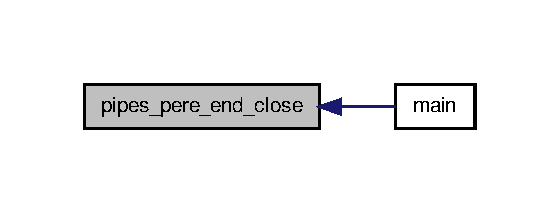
\includegraphics[width=268pt]{pipes_8h_a66dbda032de023003f32d4f4eec66875_icgraph}
\end{center}
\end{figure}


\hypertarget{pipes_8h_a7e56d9b0553fa826c8087ce2d06d987d}{\index{pipes.\-h@{pipes.\-h}!pipes\-\_\-pere\-\_\-start\-\_\-close@{pipes\-\_\-pere\-\_\-start\-\_\-close}}
\index{pipes\-\_\-pere\-\_\-start\-\_\-close@{pipes\-\_\-pere\-\_\-start\-\_\-close}!pipes.h@{pipes.\-h}}
\subsubsection[{pipes\-\_\-pere\-\_\-start\-\_\-close}]{\setlength{\rightskip}{0pt plus 5cm}int pipes\-\_\-pere\-\_\-start\-\_\-close (
\begin{DoxyParamCaption}
\item[{int $\ast$$\ast$}]{pipes}
\end{DoxyParamCaption}
)}}\label{pipes_8h_a7e56d9b0553fa826c8087ce2d06d987d}


Fermeture des pipes non utilises pour le pere. 

Ferme les pipes non utilisés du père. 
\begin{DoxyParams}{Paramètres}
{\em pipes} & Le Tableau des pipes \\
\hline
\end{DoxyParams}
\begin{DoxyReturn}{Renvoie}
Retourne 0 si tout s'est bien passé 
\end{DoxyReturn}


Définition à la ligne 107 du fichier pipes.\-c.



Voici le graphe des appelants de cette fonction \-:\nopagebreak
\begin{figure}[H]
\begin{center}
\leavevmode
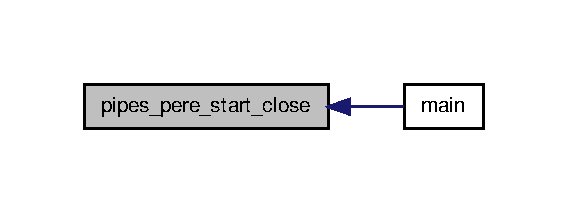
\includegraphics[width=272pt]{pipes_8h_a7e56d9b0553fa826c8087ce2d06d987d_icgraph}
\end{center}
\end{figure}



\hypertarget{regles_8h}{\section{Référence du fichier src/headers/regles.h}
\label{regles_8h}\index{src/headers/regles.\-h@{src/headers/regles.\-h}}
}


Declaration des fonctions relatives aux regles pour le jeu Petits chevaux.  


Ce graphe montre quels fichiers incluent directement ou indirectement ce fichier \-:
\nopagebreak
\begin{figure}[H]
\begin{center}
\leavevmode
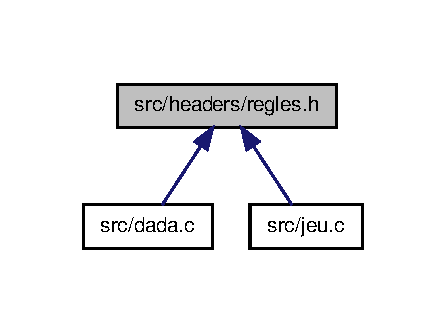
\includegraphics[width=214pt]{regles_8h__dep__incl}
\end{center}
\end{figure}
\subsection*{Fonctions}
\begin{DoxyCompactItemize}
\item 
int \hyperlink{regles_8h_a3a15257ac8021d722d70910d9eadd3b9}{cest\-\_\-mon\-\_\-tour} (int num\-\_\-fils, \hyperlink{structstruct__debuttour}{struct\-\_\-debuttour} $\ast$debuttourlu)
\begin{DoxyCompactList}\small\item\em Indique au joueur si c'est a son tour de jouer. \end{DoxyCompactList}\item 
int \hyperlink{regles_8h_a93f9bc44c4d0ed42d65c52127698963c}{nouvelle\-\_\-position} (int num\-\_\-fils, int positionjoueur, int resultatde, int $\ast$danslescalier)
\begin{DoxyCompactList}\small\item\em Donne une nouvelle position pour un joueur. \end{DoxyCompactList}\item 
int \hyperlink{regles_8h_a410ef983e618f644c9927192f5656443}{le\-\_\-joueur\-\_\-a\-\_\-gagne} (\hyperlink{structstruct__retourjeu}{struct\-\_\-retourjeu} $\ast$retourjeulu)
\begin{DoxyCompactList}\small\item\em Indique si le joueur a gagné. \end{DoxyCompactList}\item 
void \hyperlink{regles_8h_ae581f639bba80d9a02d827d6a9b94d15}{conflit\-\_\-entre\-\_\-deux\-\_\-joueur} (\hyperlink{structstruct__pendantjeu}{struct\-\_\-pendantjeu} $\ast$pendantjeulu, int $\ast$positionjoueur)
\begin{DoxyCompactList}\small\item\em Indique si il y a conflit entre deux joueurs. \end{DoxyCompactList}\item 
void \hyperlink{regles_8h_a1b36b7c7fb154d4c5402a531802c9224}{position\-\_\-escalier} (int num\-\_\-fils, int positionjoueur, int resultatde)
\end{DoxyCompactItemize}


\subsection{Description détaillée}
Declaration des fonctions relatives aux regles pour le jeu Petits chevaux. \begin{DoxyAuthor}{Auteur}
A\-O\-U\-N Abel et D\-O\-U\-C\-H\-E\-T Maximilien 
\end{DoxyAuthor}


Définition dans le fichier \hyperlink{regles_8h_source}{regles.\-h}.



\subsection{Documentation des fonctions}
\hypertarget{regles_8h_a3a15257ac8021d722d70910d9eadd3b9}{\index{regles.\-h@{regles.\-h}!cest\-\_\-mon\-\_\-tour@{cest\-\_\-mon\-\_\-tour}}
\index{cest\-\_\-mon\-\_\-tour@{cest\-\_\-mon\-\_\-tour}!regles.h@{regles.\-h}}
\subsubsection[{cest\-\_\-mon\-\_\-tour}]{\setlength{\rightskip}{0pt plus 5cm}int cest\-\_\-mon\-\_\-tour (
\begin{DoxyParamCaption}
\item[{int}]{num\-\_\-fils, }
\item[{{\bf struct\-\_\-debuttour} $\ast$}]{debuttourlu}
\end{DoxyParamCaption}
)}}\label{regles_8h_a3a15257ac8021d722d70910d9eadd3b9}


Indique au joueur si c'est a son tour de jouer. 

Celon la valeur renvoyée le joueur effectuera son tour ou non. 
\begin{DoxyParams}{Paramètres}
{\em num\-\_\-fils} & Correspond au numéro du fils appelant la fonction. \\
\hline
{\em debuttourlu} & Correspond a la structure que le joueur a recu dans le pipe par le père. \\
\hline
\end{DoxyParams}
\begin{DoxyReturn}{Renvoie}
Int Renvoie 0 si ce n'est pas au fils de jouer et 1 si c'est son tour. 
\end{DoxyReturn}


Définition à la ligne 18 du fichier regles.\-c.



Voici le graphe des appelants de cette fonction \-:\nopagebreak
\begin{figure}[H]
\begin{center}
\leavevmode
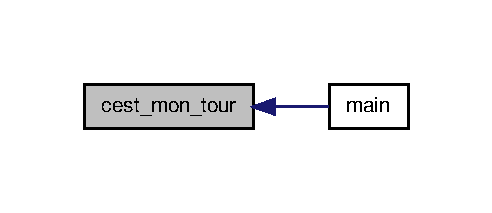
\includegraphics[width=236pt]{regles_8h_a3a15257ac8021d722d70910d9eadd3b9_icgraph}
\end{center}
\end{figure}


\hypertarget{regles_8h_ae581f639bba80d9a02d827d6a9b94d15}{\index{regles.\-h@{regles.\-h}!conflit\-\_\-entre\-\_\-deux\-\_\-joueur@{conflit\-\_\-entre\-\_\-deux\-\_\-joueur}}
\index{conflit\-\_\-entre\-\_\-deux\-\_\-joueur@{conflit\-\_\-entre\-\_\-deux\-\_\-joueur}!regles.h@{regles.\-h}}
\subsubsection[{conflit\-\_\-entre\-\_\-deux\-\_\-joueur}]{\setlength{\rightskip}{0pt plus 5cm}void conflit\-\_\-entre\-\_\-deux\-\_\-joueur (
\begin{DoxyParamCaption}
\item[{{\bf struct\-\_\-pendantjeu} $\ast$}]{pendantjeulu, }
\item[{int $\ast$}]{positionjoueur}
\end{DoxyParamCaption}
)}}\label{regles_8h_ae581f639bba80d9a02d827d6a9b94d15}


Indique si il y a conflit entre deux joueurs. 

Selon le resultat du jeu et la position des fils cela detecte et change la position d'un cavalier si il sont sur la meme case. Le nouveau cheval prend la place du précédent sur la case. Et renvoie le précédent dans l'écurie. 
\begin{DoxyParams}{Paramètres}
{\em pendantjeulu} & Structure contenant toutes les informations transmises après la phase de jeu. \\
\hline
\end{DoxyParams}
\begin{DoxyReturn}{Renvoie}
Int Renvoie 0 si il n'a pas encore gagné et 1 si il est vainqueur. 
\end{DoxyReturn}


Définition à la ligne 233 du fichier regles.\-c.



Voici le graphe des appelants de cette fonction \-:\nopagebreak
\begin{figure}[H]
\begin{center}
\leavevmode
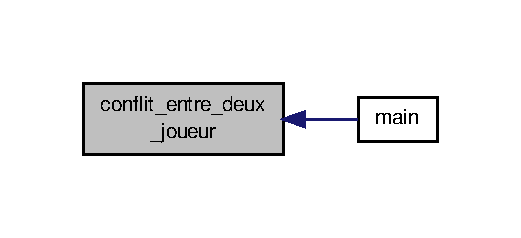
\includegraphics[width=250pt]{regles_8h_ae581f639bba80d9a02d827d6a9b94d15_icgraph}
\end{center}
\end{figure}


\hypertarget{regles_8h_a410ef983e618f644c9927192f5656443}{\index{regles.\-h@{regles.\-h}!le\-\_\-joueur\-\_\-a\-\_\-gagne@{le\-\_\-joueur\-\_\-a\-\_\-gagne}}
\index{le\-\_\-joueur\-\_\-a\-\_\-gagne@{le\-\_\-joueur\-\_\-a\-\_\-gagne}!regles.h@{regles.\-h}}
\subsubsection[{le\-\_\-joueur\-\_\-a\-\_\-gagne}]{\setlength{\rightskip}{0pt plus 5cm}int le\-\_\-joueur\-\_\-a\-\_\-gagne (
\begin{DoxyParamCaption}
\item[{{\bf struct\-\_\-retourjeu} $\ast$}]{retourjeulu}
\end{DoxyParamCaption}
)}}\label{regles_8h_a410ef983e618f644c9927192f5656443}


Indique si le joueur a gagné. 

Selon le resultat du jeu d'un fils, cela indique si ce fils a gagné 
\begin{DoxyParams}{Paramètres}
{\em retourjeulu} & Structure contenant toutes les informations importantes sur le jeu et le joueur qui vient de jouer. \\
\hline
\end{DoxyParams}
\begin{DoxyReturn}{Renvoie}
Int Renvoie 0 si il n'a pas encore gagné et 1 si il est vainqueur. 
\end{DoxyReturn}


Définition à la ligne 249 du fichier regles.\-c.



Voici le graphe des appelants de cette fonction \-:\nopagebreak
\begin{figure}[H]
\begin{center}
\leavevmode
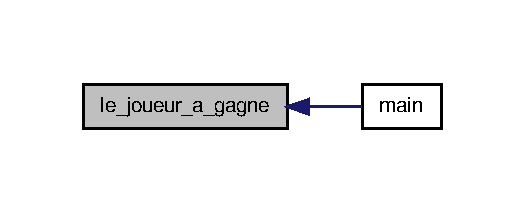
\includegraphics[width=252pt]{regles_8h_a410ef983e618f644c9927192f5656443_icgraph}
\end{center}
\end{figure}


\hypertarget{regles_8h_a93f9bc44c4d0ed42d65c52127698963c}{\index{regles.\-h@{regles.\-h}!nouvelle\-\_\-position@{nouvelle\-\_\-position}}
\index{nouvelle\-\_\-position@{nouvelle\-\_\-position}!regles.h@{regles.\-h}}
\subsubsection[{nouvelle\-\_\-position}]{\setlength{\rightskip}{0pt plus 5cm}int nouvelle\-\_\-position (
\begin{DoxyParamCaption}
\item[{int}]{num\-\_\-fils, }
\item[{int}]{positionjoueur, }
\item[{int}]{resultatde, }
\item[{int $\ast$}]{danslescalier}
\end{DoxyParamCaption}
)}}\label{regles_8h_a93f9bc44c4d0ed42d65c52127698963c}


Donne une nouvelle position pour un joueur. 

Donne une nouvelle position selon la position et le numero de joueur transmis. 
\begin{DoxyParams}{Paramètres}
{\em num\-\_\-fils} & Correspond au numéro du fils appelant la fonction. \\
\hline
{\em positionjoueur} & Correspond a la position du fils appelant la fonction. \\
\hline
{\em resultatde} & Correspond a la valeur du lance de des du joueur. \\
\hline
\end{DoxyParams}
\begin{DoxyReturn}{Renvoie}
Int Renvoie 0 si ce n'est pas au fils de jouer et 1 si c'est son tour. 
\end{DoxyReturn}


Définition à la ligne 107 du fichier regles.\-c.



Voici le graphe d'appel pour cette fonction \-:\nopagebreak
\begin{figure}[H]
\begin{center}
\leavevmode
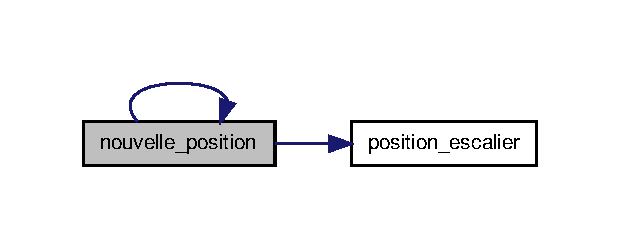
\includegraphics[width=298pt]{regles_8h_a93f9bc44c4d0ed42d65c52127698963c_cgraph}
\end{center}
\end{figure}




Voici le graphe des appelants de cette fonction \-:\nopagebreak
\begin{figure}[H]
\begin{center}
\leavevmode
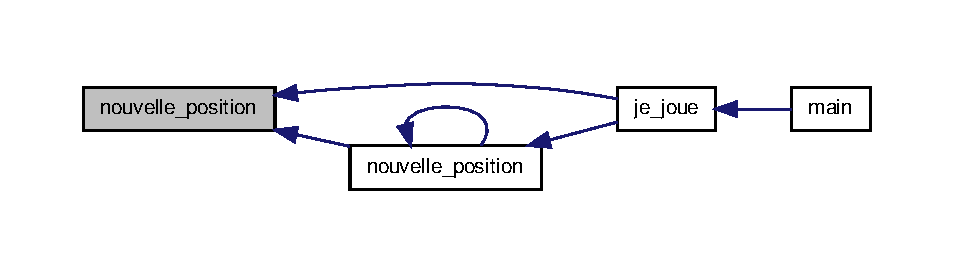
\includegraphics[width=350pt]{regles_8h_a93f9bc44c4d0ed42d65c52127698963c_icgraph}
\end{center}
\end{figure}


\hypertarget{regles_8h_a1b36b7c7fb154d4c5402a531802c9224}{\index{regles.\-h@{regles.\-h}!position\-\_\-escalier@{position\-\_\-escalier}}
\index{position\-\_\-escalier@{position\-\_\-escalier}!regles.h@{regles.\-h}}
\subsubsection[{position\-\_\-escalier}]{\setlength{\rightskip}{0pt plus 5cm}void position\-\_\-escalier (
\begin{DoxyParamCaption}
\item[{int}]{num\-\_\-fils, }
\item[{int}]{positionjoueur, }
\item[{int}]{resultatde}
\end{DoxyParamCaption}
)}}\label{regles_8h_a1b36b7c7fb154d4c5402a531802c9224}


Voici le graphe des appelants de cette fonction \-:\nopagebreak
\begin{figure}[H]
\begin{center}
\leavevmode
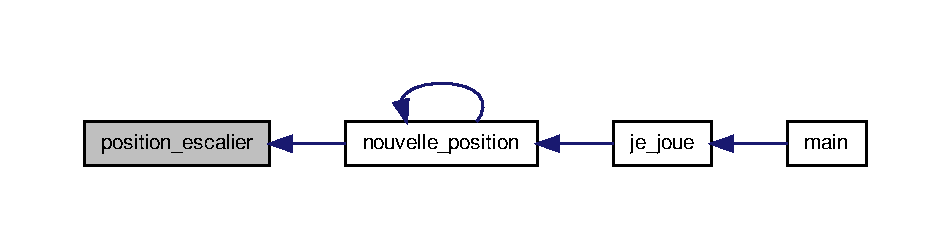
\includegraphics[width=350pt]{regles_8h_a1b36b7c7fb154d4c5402a531802c9224_icgraph}
\end{center}
\end{figure}



\hypertarget{jeu_8c}{\section{Référence du fichier src/jeu.c}
\label{jeu_8c}\index{src/jeu.\-c@{src/jeu.\-c}}
}


Fonctions relatives au jeu pour le programme Petits Chevaux.  


{\ttfamily \#include $<$stdio.\-h$>$}\\*
{\ttfamily \#include $<$stdlib.\-h$>$}\\*
{\ttfamily \#include $<$unistd.\-h$>$}\\*
{\ttfamily \#include \char`\"{}headers/jeu.\-h\char`\"{}}\\*
{\ttfamily \#include \char`\"{}headers/dada.\-h\char`\"{}}\\*
{\ttfamily \#include \char`\"{}headers/des.\-h\char`\"{}}\\*
{\ttfamily \#include \char`\"{}headers/regles.\-h\char`\"{}}\\*
\subsection*{Fonctions}
\begin{DoxyCompactItemize}
\item 
int \hyperlink{jeu_8c_aad47be4fef9e94264139f82a73b259ae}{premier\-\_\-joueur} (void)
\begin{DoxyCompactList}\small\item\em Selection par l'utilisateur du premier joueur. \end{DoxyCompactList}\item 
void \hyperlink{jeu_8c_a725da0480654655d9b7fefa6c8b8ec1d}{cest\-\_\-a\-\_\-qui\-\_\-de\-\_\-jouer} (int num\-\_\-fils, int $\ast$$\ast$pipes, \hyperlink{structstruct__debuttour}{struct\-\_\-debuttour} $\ast$debuttourlu)
\begin{DoxyCompactList}\small\item\em Recupere les informations pour le prochain tour. \end{DoxyCompactList}\item 
int \hyperlink{jeu_8c_a9b781c5cf503cd1379cd5363baf5518b}{la\-\_\-partie\-\_\-est\-\_\-interrompue} (\hyperlink{structstruct__debuttour}{struct\-\_\-debuttour} $\ast$debuttourlu)
\begin{DoxyCompactList}\small\item\em Verifie si la partie n'a pas été interrompue. \end{DoxyCompactList}\item 
int \hyperlink{jeu_8c_aae8ac69439d6ed8e1dd5b57251701a2f}{je\-\_\-joue} (int num\-\_\-fils, int $\ast$positionjoueur, \hyperlink{structstruct__pendantjeu}{struct\-\_\-pendantjeu} $\ast$pendantjeu)
\begin{DoxyCompactList}\small\item\em Action effectuées par le joueur lorsque que vient son tour. \end{DoxyCompactList}\item 
void \hyperlink{jeu_8c_a0a25bcc79238a489f286585b395ccd17}{je\-\_\-transmet\-\_\-mon\-\_\-resultat\-\_\-au\-\_\-voisin} (int num\-\_\-fils, int $\ast$$\ast$pipes, \hyperlink{structstruct__pendantjeu}{struct\-\_\-pendantjeu} $\ast$pendantjeu)
\begin{DoxyCompactList}\small\item\em Transmission des informations du jeu d'un joueurs aux autres joueurs. \end{DoxyCompactList}\item 
void \hyperlink{jeu_8c_af71947ee506f911a3e0b09dd28198e5e}{jattend\-\_\-que\-\_\-linfo\-\_\-fasse\-\_\-le\-\_\-tour} (int num\-\_\-fils, int $\ast$$\ast$pipes, \hyperlink{structstruct__pendantjeu}{struct\-\_\-pendantjeu} $\ast$pendantjeulu)
\begin{DoxyCompactList}\small\item\em Attente après envoie des informations du retour de ces informations. \end{DoxyCompactList}\item 
void \hyperlink{jeu_8c_afbccfff41a7a1c5872f6f129a8a9ab44}{je\-\_\-fais\-\_\-passer\-\_\-le\-\_\-message} (int num\-\_\-fils, int $\ast$$\ast$pipes, \hyperlink{structstruct__pendantjeu}{struct\-\_\-pendantjeu} $\ast$pendantjeulu)
\begin{DoxyCompactList}\small\item\em Fait passer les informations au suivant. \end{DoxyCompactList}\item 
void \hyperlink{jeu_8c_aedc8c2b1001e2680710ac7ef3d73cac8}{je\-\_\-transmet\-\_\-mon\-\_\-resultat\-\_\-au\-\_\-pere} (int num\-\_\-fils, int $\ast$$\ast$pipes, \hyperlink{structstruct__retourjeu}{struct\-\_\-retourjeu} $\ast$retourjeu, int resultatde, int positionjoueur)
\begin{DoxyCompactList}\small\item\em Transmet les informations au père. \end{DoxyCompactList}\item 
void \hyperlink{jeu_8c_a2a267585992923972c7c142df69c5b89}{pere\-\_\-envoyer\-\_\-message\-\_\-aux\-\_\-fils} (int $\ast$$\ast$pipes, \hyperlink{structstruct__debuttour}{struct\-\_\-debuttour} $\ast$debuttour, int numerojoueur, int partieencours)
\begin{DoxyCompactList}\small\item\em Transmet les informations du père vers les fils. \end{DoxyCompactList}\item 
void \hyperlink{jeu_8c_a96da99031da1d74f38b559243dad2171}{pere\-\_\-lit\-\_\-retour\-\_\-tour} (int $\ast$$\ast$pipes, \hyperlink{structstruct__retourjeu}{struct\-\_\-retourjeu} $\ast$retourjeulu)
\begin{DoxyCompactList}\small\item\em Lecture des informations transmises par les fils. \end{DoxyCompactList}\item 
int \hyperlink{jeu_8c_ab99f683f90789787a7d8201407214cc1}{joueur\-\_\-suivant} (\hyperlink{structstruct__retourjeu}{struct\-\_\-retourjeu} $\ast$retourjeulu)
\begin{DoxyCompactList}\small\item\em Indique le prochain joueur devant jouer. \end{DoxyCompactList}\end{DoxyCompactItemize}


\subsection{Description détaillée}
Fonctions relatives au jeu pour le programme Petits Chevaux. \begin{DoxyAuthor}{Auteur}
A\-O\-U\-N Abel et D\-O\-U\-C\-H\-E\-T Maximilien 
\end{DoxyAuthor}


\subsection{Documentation des fonctions}
\hypertarget{jeu_8c_a725da0480654655d9b7fefa6c8b8ec1d}{\index{jeu.\-c@{jeu.\-c}!cest\-\_\-a\-\_\-qui\-\_\-de\-\_\-jouer@{cest\-\_\-a\-\_\-qui\-\_\-de\-\_\-jouer}}
\index{cest\-\_\-a\-\_\-qui\-\_\-de\-\_\-jouer@{cest\-\_\-a\-\_\-qui\-\_\-de\-\_\-jouer}!jeu.c@{jeu.\-c}}
\subsubsection[{cest\-\_\-a\-\_\-qui\-\_\-de\-\_\-jouer}]{\setlength{\rightskip}{0pt plus 5cm}void cest\-\_\-a\-\_\-qui\-\_\-de\-\_\-jouer (
\begin{DoxyParamCaption}
\item[{int}]{num\-\_\-fils, }
\item[{int $\ast$$\ast$}]{pipes, }
\item[{{\bf struct\-\_\-debuttour} $\ast$}]{debuttourlu}
\end{DoxyParamCaption}
)}}\label{jeu_8c_a725da0480654655d9b7fefa6c8b8ec1d}


Recupere les informations pour le prochain tour. 

Récupère dans le pipe venant du main vers le joueur concerné la structure contenant les informations pour le prochain tour. 
\begin{DoxyParams}{Paramètres}
{\em num\-\_\-fils} & Int -\/ Correspond au numéro du fils souhaitant récupérer les informations. \\
\hline
{\em pipes} & Tableau des pipes. \\
\hline
{\em debuttourlu} & Pointeur sur la structure. \\
\hline
\end{DoxyParams}
\begin{DoxyReturn}{Renvoie}
Void 
\end{DoxyReturn}
\hypertarget{jeu_8c_af71947ee506f911a3e0b09dd28198e5e}{\index{jeu.\-c@{jeu.\-c}!jattend\-\_\-que\-\_\-linfo\-\_\-fasse\-\_\-le\-\_\-tour@{jattend\-\_\-que\-\_\-linfo\-\_\-fasse\-\_\-le\-\_\-tour}}
\index{jattend\-\_\-que\-\_\-linfo\-\_\-fasse\-\_\-le\-\_\-tour@{jattend\-\_\-que\-\_\-linfo\-\_\-fasse\-\_\-le\-\_\-tour}!jeu.c@{jeu.\-c}}
\subsubsection[{jattend\-\_\-que\-\_\-linfo\-\_\-fasse\-\_\-le\-\_\-tour}]{\setlength{\rightskip}{0pt plus 5cm}void jattend\-\_\-que\-\_\-linfo\-\_\-fasse\-\_\-le\-\_\-tour (
\begin{DoxyParamCaption}
\item[{int}]{num\-\_\-fils, }
\item[{int $\ast$$\ast$}]{pipes, }
\item[{{\bf struct\-\_\-pendantjeu} $\ast$}]{pendantjeulu}
\end{DoxyParamCaption}
)}}\label{jeu_8c_af71947ee506f911a3e0b09dd28198e5e}


Attente après envoie des informations du retour de ces informations. 

Permet la récupération des informations envoyés par le biais du joueur précédent. Ce en lisant dans le pipe du joueur précédent le num\-\_\-fils. Quand l'information sera revenue, elle aura fait le tour. 
\begin{DoxyParams}{Paramètres}
{\em num\-\_\-fils} & Int -\/ Correspond au numéro du fils souhaitant récupérer les informations. \\
\hline
{\em pipes} & Tableau des pipes. \\
\hline
{\em pendantjeulu} & Pointeur sur la structure contenant les informations du jeu qui vient d'être fait et transmis par le voisin précédent. \\
\hline
\end{DoxyParams}
\begin{DoxyReturn}{Renvoie}
Void -\/ Termine en cas d'erreur 
\end{DoxyReturn}
\hypertarget{jeu_8c_afbccfff41a7a1c5872f6f129a8a9ab44}{\index{jeu.\-c@{jeu.\-c}!je\-\_\-fais\-\_\-passer\-\_\-le\-\_\-message@{je\-\_\-fais\-\_\-passer\-\_\-le\-\_\-message}}
\index{je\-\_\-fais\-\_\-passer\-\_\-le\-\_\-message@{je\-\_\-fais\-\_\-passer\-\_\-le\-\_\-message}!jeu.c@{jeu.\-c}}
\subsubsection[{je\-\_\-fais\-\_\-passer\-\_\-le\-\_\-message}]{\setlength{\rightskip}{0pt plus 5cm}void je\-\_\-fais\-\_\-passer\-\_\-le\-\_\-message (
\begin{DoxyParamCaption}
\item[{int}]{num\-\_\-fils, }
\item[{int $\ast$$\ast$}]{pipes, }
\item[{{\bf struct\-\_\-pendantjeu} $\ast$}]{pendantjeulu}
\end{DoxyParamCaption}
)}}\label{jeu_8c_afbccfff41a7a1c5872f6f129a8a9ab44}


Fait passer les informations au suivant. 

Permet la transmission des informations envoyés par le biais du joueur précédent. Ce en lisant dans le pipe du joueur précédent le num\-\_\-fils. On l'envoie au suivant immédiatement. Cela nous permet d'appliquer la regle pour que le joueur revienne au point de départ si un autre joueur est arrivé sur la même case. Cette fonction est appellée lorsque ce n'est pas à num\-\_\-fils de jouer. 
\begin{DoxyParams}{Paramètres}
{\em num\-\_\-fils} & Int -\/ Correspond au numéro du fils souhaitant récupérer les informations. \\
\hline
{\em pipes} & Tableau des pipes. \\
\hline
{\em pendantjeulu} & Pointeur sur la structure contenant les informations du jeu qui vient d'être transmis par le voisin précédent. \\
\hline
\end{DoxyParams}
\begin{DoxyReturn}{Renvoie}
Void -\/ Termine en cas d'erreur 
\end{DoxyReturn}
\hypertarget{jeu_8c_aae8ac69439d6ed8e1dd5b57251701a2f}{\index{jeu.\-c@{jeu.\-c}!je\-\_\-joue@{je\-\_\-joue}}
\index{je\-\_\-joue@{je\-\_\-joue}!jeu.c@{jeu.\-c}}
\subsubsection[{je\-\_\-joue}]{\setlength{\rightskip}{0pt plus 5cm}int je\-\_\-joue (
\begin{DoxyParamCaption}
\item[{int}]{num\-\_\-fils, }
\item[{int $\ast$}]{positionjoueur, }
\item[{{\bf struct\-\_\-pendantjeu} $\ast$}]{pendantjeu}
\end{DoxyParamCaption}
)}}\label{jeu_8c_aae8ac69439d6ed8e1dd5b57251701a2f}


Action effectuées par le joueur lorsque que vient son tour. 

Le joueur lance un dé, demande aux reglès quelle est sa nouvelle position et enregistre ces informations. 
\begin{DoxyParams}{Paramètres}
{\em num\-\_\-fils} & Int -\/ Correspond au numéro du fils souhaitant récupérer les informations. \\
\hline
{\em positionjoueur} & Pointeur sur la position du joueur appelant la fonction. \\
\hline
{\em pendantjeu} & Pointeur sur la structure qui va être transmise aux autres joueurs. \\
\hline
\end{DoxyParams}
\begin{DoxyReturn}{Renvoie}
Int -\/ Retourne le resultat du lancé de dé, la position est déjà modifiée. 
\end{DoxyReturn}
\hypertarget{jeu_8c_aedc8c2b1001e2680710ac7ef3d73cac8}{\index{jeu.\-c@{jeu.\-c}!je\-\_\-transmet\-\_\-mon\-\_\-resultat\-\_\-au\-\_\-pere@{je\-\_\-transmet\-\_\-mon\-\_\-resultat\-\_\-au\-\_\-pere}}
\index{je\-\_\-transmet\-\_\-mon\-\_\-resultat\-\_\-au\-\_\-pere@{je\-\_\-transmet\-\_\-mon\-\_\-resultat\-\_\-au\-\_\-pere}!jeu.c@{jeu.\-c}}
\subsubsection[{je\-\_\-transmet\-\_\-mon\-\_\-resultat\-\_\-au\-\_\-pere}]{\setlength{\rightskip}{0pt plus 5cm}void je\-\_\-transmet\-\_\-mon\-\_\-resultat\-\_\-au\-\_\-pere (
\begin{DoxyParamCaption}
\item[{int}]{num\-\_\-fils, }
\item[{int $\ast$$\ast$}]{pipes, }
\item[{{\bf struct\-\_\-retourjeu} $\ast$}]{retourjeu, }
\item[{int}]{resultatde, }
\item[{int}]{positionjoueur}
\end{DoxyParamCaption}
)}}\label{jeu_8c_aedc8c2b1001e2680710ac7ef3d73cac8}


Transmet les informations au père. 

Quand les informations transmises ont fait le tour, on génère une structure contenant les informations dont le père aura besoin pour modérer. On lui envoie alors dans le pipe des fils vers le père. 
\begin{DoxyParams}{Paramètres}
{\em num\-\_\-fils} & Int -\/ Correspond au numéro du fils souhaitant récupérer les informations. \\
\hline
{\em pipes} & Tableau des pipes. \\
\hline
{\em retourjeu} & Pointeur sur la structure contenant les informations du jeu qui vient d'être fait et ayant fait le tour. \\
\hline
{\em resultatde} & Valeur du dé lancé. Utile pour le père afin de savoir si le fils doit rejouer ou non. En cas de double 6. \\
\hline
{\em positionjoueur} & Nouvelle position du joueur. Utile pour savoir si un joueur est arrivé au bout de sa course. \\
\hline
\end{DoxyParams}
\begin{DoxyReturn}{Renvoie}
Void -\/ Termine en cas d'erreur 
\end{DoxyReturn}
\hypertarget{jeu_8c_a0a25bcc79238a489f286585b395ccd17}{\index{jeu.\-c@{jeu.\-c}!je\-\_\-transmet\-\_\-mon\-\_\-resultat\-\_\-au\-\_\-voisin@{je\-\_\-transmet\-\_\-mon\-\_\-resultat\-\_\-au\-\_\-voisin}}
\index{je\-\_\-transmet\-\_\-mon\-\_\-resultat\-\_\-au\-\_\-voisin@{je\-\_\-transmet\-\_\-mon\-\_\-resultat\-\_\-au\-\_\-voisin}!jeu.c@{jeu.\-c}}
\subsubsection[{je\-\_\-transmet\-\_\-mon\-\_\-resultat\-\_\-au\-\_\-voisin}]{\setlength{\rightskip}{0pt plus 5cm}void je\-\_\-transmet\-\_\-mon\-\_\-resultat\-\_\-au\-\_\-voisin (
\begin{DoxyParamCaption}
\item[{int}]{num\-\_\-fils, }
\item[{int $\ast$$\ast$}]{pipes, }
\item[{{\bf struct\-\_\-pendantjeu} $\ast$}]{pendantjeu}
\end{DoxyParamCaption}
)}}\label{jeu_8c_a0a25bcc79238a489f286585b395ccd17}


Transmission des informations du jeu d'un joueurs aux autres joueurs. 

La structure contenant les informations du jeu qui vient d'être effectué est déjà crée. Il ne reste qu'a l'écrire dans le pipe du voisin. 
\begin{DoxyParams}{Paramètres}
{\em num\-\_\-fils} & Int -\/ Correspond au numéro du fils souhaitant récupérer les informations. \\
\hline
{\em pipes} & Tableau des pipes. \\
\hline
{\em pendantjeu} & Pointeur sur la structure contenant les informations du jeu qui vient d'être fait. \\
\hline
\end{DoxyParams}
\begin{DoxyReturn}{Renvoie}
Void -\/ Termine en cas d'erreur 
\end{DoxyReturn}
\hypertarget{jeu_8c_ab99f683f90789787a7d8201407214cc1}{\index{jeu.\-c@{jeu.\-c}!joueur\-\_\-suivant@{joueur\-\_\-suivant}}
\index{joueur\-\_\-suivant@{joueur\-\_\-suivant}!jeu.c@{jeu.\-c}}
\subsubsection[{joueur\-\_\-suivant}]{\setlength{\rightskip}{0pt plus 5cm}int joueur\-\_\-suivant (
\begin{DoxyParamCaption}
\item[{{\bf struct\-\_\-retourjeu} $\ast$}]{retourjeulu}
\end{DoxyParamCaption}
)}}\label{jeu_8c_ab99f683f90789787a7d8201407214cc1}


Indique le prochain joueur devant jouer. 

Selon le retour des informations renvoyées au père après un tour de jeu. Le père décide si il fait rejouer un joueur (en cas de double 6), ou si il donne la main au suivant. 
\begin{DoxyParams}{Paramètres}
{\em retourjeulu} & Pointeur sur la structure devant contenir les informations destinées au père par le joueurs. \\
\hline
\end{DoxyParams}
\begin{DoxyReturn}{Renvoie}
result Int -\/ Le numéro du prochain joueur devant s'executer. 
\end{DoxyReturn}
\hypertarget{jeu_8c_a9b781c5cf503cd1379cd5363baf5518b}{\index{jeu.\-c@{jeu.\-c}!la\-\_\-partie\-\_\-est\-\_\-interrompue@{la\-\_\-partie\-\_\-est\-\_\-interrompue}}
\index{la\-\_\-partie\-\_\-est\-\_\-interrompue@{la\-\_\-partie\-\_\-est\-\_\-interrompue}!jeu.c@{jeu.\-c}}
\subsubsection[{la\-\_\-partie\-\_\-est\-\_\-interrompue}]{\setlength{\rightskip}{0pt plus 5cm}int la\-\_\-partie\-\_\-est\-\_\-interrompue (
\begin{DoxyParamCaption}
\item[{{\bf struct\-\_\-debuttour} $\ast$}]{debuttourlu}
\end{DoxyParamCaption}
)}}\label{jeu_8c_a9b781c5cf503cd1379cd5363baf5518b}


Verifie si la partie n'a pas été interrompue. 

Dans le cas ou un joueur a gagné, nous considérons que la partie est finie. Dans le cas ou l'utilisateur choisi d'interrompre le programme cette fonction sera très utile pour permettre aux joueurs de se tuer même si ils n'ont pas fini de jouer. 
\begin{DoxyParams}{Paramètres}
{\em debuttourlu} & Pointeur sur la structure lue au debut du tour. \\
\hline
\end{DoxyParams}
\begin{DoxyReturn}{Renvoie}
Int -\/ Renvoie 1 si la partie est termine ou interrompue, 0 sinon. 
\end{DoxyReturn}
\hypertarget{jeu_8c_a2a267585992923972c7c142df69c5b89}{\index{jeu.\-c@{jeu.\-c}!pere\-\_\-envoyer\-\_\-message\-\_\-aux\-\_\-fils@{pere\-\_\-envoyer\-\_\-message\-\_\-aux\-\_\-fils}}
\index{pere\-\_\-envoyer\-\_\-message\-\_\-aux\-\_\-fils@{pere\-\_\-envoyer\-\_\-message\-\_\-aux\-\_\-fils}!jeu.c@{jeu.\-c}}
\subsubsection[{pere\-\_\-envoyer\-\_\-message\-\_\-aux\-\_\-fils}]{\setlength{\rightskip}{0pt plus 5cm}void pere\-\_\-envoyer\-\_\-message\-\_\-aux\-\_\-fils (
\begin{DoxyParamCaption}
\item[{int $\ast$$\ast$}]{pipes, }
\item[{{\bf struct\-\_\-debuttour} $\ast$}]{debuttour, }
\item[{int}]{numerojoueur, }
\item[{int}]{partieencours}
\end{DoxyParamCaption}
)}}\label{jeu_8c_a2a267585992923972c7c142df69c5b89}


Transmet les informations du père vers les fils. 

Quand les informations transmises au père ont été analysé, ou lors du premier tour le père doit envoyer des informations au fils. 
\begin{DoxyParams}{Paramètres}
{\em pipes} & Tableau des pipes. \\
\hline
{\em debuttour} & Pointeur sur la structure devant contenir les informations qui vont être transmises au joueur. \\
\hline
{\em numerojoueur} & Numéro du prochain joueur devant jouer. \\
\hline
{\em partieencours} & Indique si la partie est toujours en cours. (1 oui $|$ 0 -\/ non) \\
\hline
\end{DoxyParams}
\begin{DoxyReturn}{Renvoie}
Void -\/ Termine en cas d'erreur 
\end{DoxyReturn}
\hypertarget{jeu_8c_a96da99031da1d74f38b559243dad2171}{\index{jeu.\-c@{jeu.\-c}!pere\-\_\-lit\-\_\-retour\-\_\-tour@{pere\-\_\-lit\-\_\-retour\-\_\-tour}}
\index{pere\-\_\-lit\-\_\-retour\-\_\-tour@{pere\-\_\-lit\-\_\-retour\-\_\-tour}!jeu.c@{jeu.\-c}}
\subsubsection[{pere\-\_\-lit\-\_\-retour\-\_\-tour}]{\setlength{\rightskip}{0pt plus 5cm}void pere\-\_\-lit\-\_\-retour\-\_\-tour (
\begin{DoxyParamCaption}
\item[{int $\ast$$\ast$}]{pipes, }
\item[{{\bf struct\-\_\-retourjeu} $\ast$}]{retourjeulu}
\end{DoxyParamCaption}
)}}\label{jeu_8c_a96da99031da1d74f38b559243dad2171}


Lecture des informations transmises par les fils. 

Le joueur qui vient de jouer fait remonter des informations au père une fois qu'il vient de terminer de faire circuler des informations aux autres joueurs. 
\begin{DoxyParams}{Paramètres}
{\em pipes} & Tableau des pipes. \\
\hline
{\em retourjeulu} & Pointeur sur la structure devant contenir les informations destinées au père par le joueurs. \\
\hline
\end{DoxyParams}
\begin{DoxyReturn}{Renvoie}
Void -\/ Termine en cas d'erreur 
\end{DoxyReturn}
\hypertarget{jeu_8c_aad47be4fef9e94264139f82a73b259ae}{\index{jeu.\-c@{jeu.\-c}!premier\-\_\-joueur@{premier\-\_\-joueur}}
\index{premier\-\_\-joueur@{premier\-\_\-joueur}!jeu.c@{jeu.\-c}}
\subsubsection[{premier\-\_\-joueur}]{\setlength{\rightskip}{0pt plus 5cm}int premier\-\_\-joueur (
\begin{DoxyParamCaption}
\item[{void}]{}
\end{DoxyParamCaption}
)}}\label{jeu_8c_aad47be4fef9e94264139f82a73b259ae}


Selection par l'utilisateur du premier joueur. 

Demande a l'utilisateur de saisir le numero du premier joueur. \begin{DoxyReturn}{Renvoie}
Int -\/ Retourne le numero du joueur saisi. 
\end{DoxyReturn}

\hypertarget{pipes_8c}{\section{Référence du fichier src/pipes.c}
\label{pipes_8c}\index{src/pipes.\-c@{src/pipes.\-c}}
}


Fonctions relatives au pipes pour le jeu Petits chevaux.  


{\ttfamily \#include $<$stdio.\-h$>$}\\*
{\ttfamily \#include $<$stdlib.\-h$>$}\\*
{\ttfamily \#include $<$unistd.\-h$>$}\\*
Graphe des dépendances par inclusion de pipes.\-c\-:
\nopagebreak
\begin{figure}[H]
\begin{center}
\leavevmode
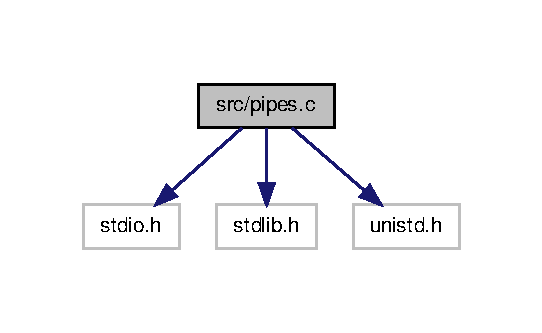
\includegraphics[width=260pt]{pipes_8c__incl}
\end{center}
\end{figure}
\subsection*{Fonctions}
\begin{DoxyCompactItemize}
\item 
int \hyperlink{pipes_8c_a8efe620a19ac0e4f120345e57b6edeac}{creation\-\_\-pipes} (int $\ast$$\ast$pipes)
\begin{DoxyCompactList}\small\item\em Creation des pipes. \end{DoxyCompactList}\item 
int \hyperlink{pipes_8c_a4352c1ccc165cf89b0c4d6a748b1dd58}{pipes\-\_\-fils\-\_\-start\-\_\-close} (int num\-\_\-fils, int $\ast$$\ast$pipes)
\begin{DoxyCompactList}\small\item\em Fermeture des pipes non utilises pour chaque fils. \end{DoxyCompactList}\item 
int \hyperlink{pipes_8c_a07068e6f96cddd3caeaa6dde747270e7}{pipes\-\_\-fils\-\_\-end\-\_\-close} (int num\-\_\-fils, int $\ast$$\ast$pipes)
\begin{DoxyCompactList}\small\item\em Fermeture des pipes utilisés pour chaque fils. \end{DoxyCompactList}\item 
int \hyperlink{pipes_8c_a7e56d9b0553fa826c8087ce2d06d987d}{pipes\-\_\-pere\-\_\-start\-\_\-close} (int $\ast$$\ast$pipes)
\begin{DoxyCompactList}\small\item\em Fermeture des pipes non utilises pour le pere. \end{DoxyCompactList}\item 
int \hyperlink{pipes_8c_a66dbda032de023003f32d4f4eec66875}{pipes\-\_\-pere\-\_\-end\-\_\-close} (int $\ast$$\ast$pipes)
\begin{DoxyCompactList}\small\item\em Fermeture des pipes utilisés pour le père. \end{DoxyCompactList}\end{DoxyCompactItemize}


\subsection{Description détaillée}
Fonctions relatives au pipes pour le jeu Petits chevaux. \begin{DoxyAuthor}{Auteur}
A\-O\-U\-N Abel et D\-O\-U\-C\-H\-E\-T Maximilien
\end{DoxyAuthor}
Les pipes sont organisés de cette maniere \-: 0 -\/$>$ Entree du main depuis joueurs 1 -\/$>$ sortie du main vers joueur 1 2 -\/$>$ sortie du main vers joueur 2 3 -\/$>$ sortie du main vers joueur 3 4 -\/$>$ sortie du main vers joueur 4 5 -\/$>$ sortie du joueur 1 vers joueur 2 6 -\/$>$ sortie du joueur 2 vers joueur 3 7 -\/$>$ sortie du joueur 3 vers joueur 4 8 -\/$>$ sortie du joueur 4 vers joueur 1 

Définition dans le fichier \hyperlink{pipes_8c_source}{pipes.\-c}.



\subsection{Documentation des fonctions}
\hypertarget{pipes_8c_a8efe620a19ac0e4f120345e57b6edeac}{\index{pipes.\-c@{pipes.\-c}!creation\-\_\-pipes@{creation\-\_\-pipes}}
\index{creation\-\_\-pipes@{creation\-\_\-pipes}!pipes.c@{pipes.\-c}}
\subsubsection[{creation\-\_\-pipes}]{\setlength{\rightskip}{0pt plus 5cm}int creation\-\_\-pipes (
\begin{DoxyParamCaption}
\item[{int $\ast$$\ast$}]{pipes}
\end{DoxyParamCaption}
)}}\label{pipes_8c_a8efe620a19ac0e4f120345e57b6edeac}


Creation des pipes. 

Fonction de creation des pipes 
\begin{DoxyParams}{Paramètres}
{\em pipes} & Tableau des pipes \\
\hline
\end{DoxyParams}
\begin{DoxyReturn}{Renvoie}
Retourne 0 si tout s'est bien passé 
\end{DoxyReturn}


Définition à la ligne 28 du fichier pipes.\-c.



Voici le graphe des appelants de cette fonction \-:
\nopagebreak
\begin{figure}[H]
\begin{center}
\leavevmode
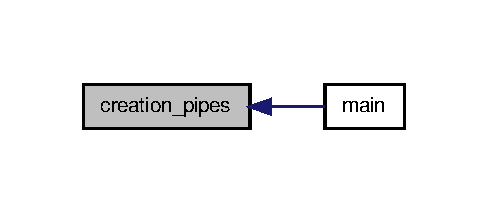
\includegraphics[width=234pt]{pipes_8c_a8efe620a19ac0e4f120345e57b6edeac_icgraph}
\end{center}
\end{figure}


\hypertarget{pipes_8c_a07068e6f96cddd3caeaa6dde747270e7}{\index{pipes.\-c@{pipes.\-c}!pipes\-\_\-fils\-\_\-end\-\_\-close@{pipes\-\_\-fils\-\_\-end\-\_\-close}}
\index{pipes\-\_\-fils\-\_\-end\-\_\-close@{pipes\-\_\-fils\-\_\-end\-\_\-close}!pipes.c@{pipes.\-c}}
\subsubsection[{pipes\-\_\-fils\-\_\-end\-\_\-close}]{\setlength{\rightskip}{0pt plus 5cm}int pipes\-\_\-fils\-\_\-end\-\_\-close (
\begin{DoxyParamCaption}
\item[{int}]{num\-\_\-fils, }
\item[{int $\ast$$\ast$}]{pipes}
\end{DoxyParamCaption}
)}}\label{pipes_8c_a07068e6f96cddd3caeaa6dde747270e7}


Fermeture des pipes utilisés pour chaque fils. 

Ferme les pipes de chaque fils utilisés lorsque qu'il n'en a plus besoin. 
\begin{DoxyParams}{Paramètres}
{\em num\-\_\-fils} & Le numéro du fils souhaitant fermer ses pipes \\
\hline
{\em pipes} & Le Tableau des pipes \\
\hline
\end{DoxyParams}
\begin{DoxyReturn}{Renvoie}
Retourne 0 si tout s'est bien passé 
\end{DoxyReturn}


Définition à la ligne 82 du fichier pipes.\-c.



Voici le graphe des appelants de cette fonction \-:
\nopagebreak
\begin{figure}[H]
\begin{center}
\leavevmode
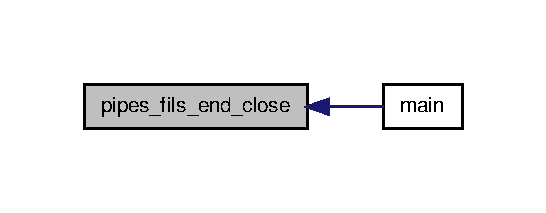
\includegraphics[width=262pt]{pipes_8c_a07068e6f96cddd3caeaa6dde747270e7_icgraph}
\end{center}
\end{figure}


\hypertarget{pipes_8c_a4352c1ccc165cf89b0c4d6a748b1dd58}{\index{pipes.\-c@{pipes.\-c}!pipes\-\_\-fils\-\_\-start\-\_\-close@{pipes\-\_\-fils\-\_\-start\-\_\-close}}
\index{pipes\-\_\-fils\-\_\-start\-\_\-close@{pipes\-\_\-fils\-\_\-start\-\_\-close}!pipes.c@{pipes.\-c}}
\subsubsection[{pipes\-\_\-fils\-\_\-start\-\_\-close}]{\setlength{\rightskip}{0pt plus 5cm}int pipes\-\_\-fils\-\_\-start\-\_\-close (
\begin{DoxyParamCaption}
\item[{int}]{num\-\_\-fils, }
\item[{int $\ast$$\ast$}]{pipes}
\end{DoxyParamCaption}
)}}\label{pipes_8c_a4352c1ccc165cf89b0c4d6a748b1dd58}


Fermeture des pipes non utilises pour chaque fils. 

Ferme les pipes de chaque fils non utilisés. 
\begin{DoxyParams}{Paramètres}
{\em num\-\_\-fils} & Le numéro du fils souhaitant fermer ses pipes \\
\hline
{\em pipes} & Le Tableau des pipes \\
\hline
\end{DoxyParams}
\begin{DoxyReturn}{Renvoie}
Retourne 0 si tout s'est bien passé 
\end{DoxyReturn}


Définition à la ligne 47 du fichier pipes.\-c.



Voici le graphe des appelants de cette fonction \-:
\nopagebreak
\begin{figure}[H]
\begin{center}
\leavevmode
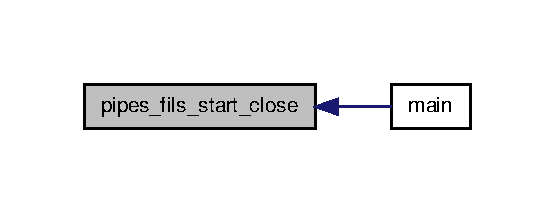
\includegraphics[width=266pt]{pipes_8c_a4352c1ccc165cf89b0c4d6a748b1dd58_icgraph}
\end{center}
\end{figure}


\hypertarget{pipes_8c_a66dbda032de023003f32d4f4eec66875}{\index{pipes.\-c@{pipes.\-c}!pipes\-\_\-pere\-\_\-end\-\_\-close@{pipes\-\_\-pere\-\_\-end\-\_\-close}}
\index{pipes\-\_\-pere\-\_\-end\-\_\-close@{pipes\-\_\-pere\-\_\-end\-\_\-close}!pipes.c@{pipes.\-c}}
\subsubsection[{pipes\-\_\-pere\-\_\-end\-\_\-close}]{\setlength{\rightskip}{0pt plus 5cm}int pipes\-\_\-pere\-\_\-end\-\_\-close (
\begin{DoxyParamCaption}
\item[{int $\ast$$\ast$}]{pipes}
\end{DoxyParamCaption}
)}}\label{pipes_8c_a66dbda032de023003f32d4f4eec66875}


Fermeture des pipes utilisés pour le père. 

Ferme les pipes du père utilisés lorsque qu'il n'en a plus besoin. 
\begin{DoxyParams}{Paramètres}
{\em pipes} & Le Tableau des pipes \\
\hline
\end{DoxyParams}
\begin{DoxyReturn}{Renvoie}
Retourne 0 si tout s'est bien passé 
\end{DoxyReturn}


Définition à la ligne 131 du fichier pipes.\-c.



Voici le graphe des appelants de cette fonction \-:
\nopagebreak
\begin{figure}[H]
\begin{center}
\leavevmode
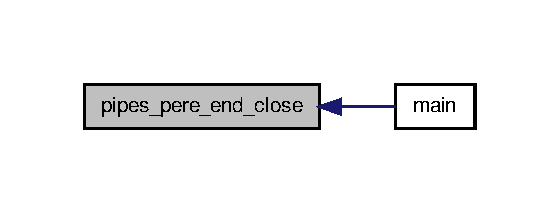
\includegraphics[width=268pt]{pipes_8c_a66dbda032de023003f32d4f4eec66875_icgraph}
\end{center}
\end{figure}


\hypertarget{pipes_8c_a7e56d9b0553fa826c8087ce2d06d987d}{\index{pipes.\-c@{pipes.\-c}!pipes\-\_\-pere\-\_\-start\-\_\-close@{pipes\-\_\-pere\-\_\-start\-\_\-close}}
\index{pipes\-\_\-pere\-\_\-start\-\_\-close@{pipes\-\_\-pere\-\_\-start\-\_\-close}!pipes.c@{pipes.\-c}}
\subsubsection[{pipes\-\_\-pere\-\_\-start\-\_\-close}]{\setlength{\rightskip}{0pt plus 5cm}int pipes\-\_\-pere\-\_\-start\-\_\-close (
\begin{DoxyParamCaption}
\item[{int $\ast$$\ast$}]{pipes}
\end{DoxyParamCaption}
)}}\label{pipes_8c_a7e56d9b0553fa826c8087ce2d06d987d}


Fermeture des pipes non utilises pour le pere. 

Ferme les pipes non utilisés du père. 
\begin{DoxyParams}{Paramètres}
{\em pipes} & Le Tableau des pipes \\
\hline
\end{DoxyParams}
\begin{DoxyReturn}{Renvoie}
Retourne 0 si tout s'est bien passé 
\end{DoxyReturn}


Définition à la ligne 107 du fichier pipes.\-c.



Voici le graphe des appelants de cette fonction \-:
\nopagebreak
\begin{figure}[H]
\begin{center}
\leavevmode
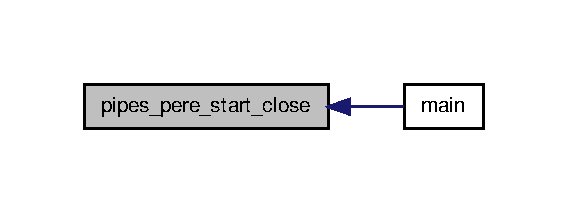
\includegraphics[width=272pt]{pipes_8c_a7e56d9b0553fa826c8087ce2d06d987d_icgraph}
\end{center}
\end{figure}



\hypertarget{regles_8c}{\section{Référence du fichier src/regles.c}
\label{regles_8c}\index{src/regles.\-c@{src/regles.\-c}}
}


Fonctions relatives aux regles pour le jeu Petits chevaux.  


{\ttfamily \#include $<$stdio.\-h$>$}\\*
{\ttfamily \#include \char`\"{}headers/jeu.\-h\char`\"{}}\\*
\subsection*{Fonctions}
\begin{DoxyCompactItemize}
\item 
int \hyperlink{regles_8c_a3a15257ac8021d722d70910d9eadd3b9}{cest\-\_\-mon\-\_\-tour} (int num\-\_\-fils, \hyperlink{structstruct__debuttour}{struct\-\_\-debuttour} $\ast$debuttourlu)
\begin{DoxyCompactList}\small\item\em Indique au joueur si c'est a son tour de jouer. \end{DoxyCompactList}\item 
int \hyperlink{regles_8c_a14d8af584e9671d7a2f9ba56838f4672}{nouvelle\-\_\-position} (int num\-\_\-fils, int positionjoueur, int resultatde)
\begin{DoxyCompactList}\small\item\em Donne une nouvelle position pour un joueur. \end{DoxyCompactList}\item 
int \hyperlink{regles_8c_a410ef983e618f644c9927192f5656443}{le\-\_\-joueur\-\_\-a\-\_\-gagne} (\hyperlink{structstruct__retourjeu}{struct\-\_\-retourjeu} $\ast$retourjeulu)
\begin{DoxyCompactList}\small\item\em Indique si le joueur a gagné. \end{DoxyCompactList}\end{DoxyCompactItemize}


\subsection{Description détaillée}
Fonctions relatives aux regles pour le jeu Petits chevaux. \begin{DoxyAuthor}{Auteur}
A\-O\-U\-N Abel et D\-O\-U\-C\-H\-E\-T Maximilien 
\end{DoxyAuthor}


\subsection{Documentation des fonctions}
\hypertarget{regles_8c_a3a15257ac8021d722d70910d9eadd3b9}{\index{regles.\-c@{regles.\-c}!cest\-\_\-mon\-\_\-tour@{cest\-\_\-mon\-\_\-tour}}
\index{cest\-\_\-mon\-\_\-tour@{cest\-\_\-mon\-\_\-tour}!regles.c@{regles.\-c}}
\subsubsection[{cest\-\_\-mon\-\_\-tour}]{\setlength{\rightskip}{0pt plus 5cm}int cest\-\_\-mon\-\_\-tour (
\begin{DoxyParamCaption}
\item[{int}]{num\-\_\-fils, }
\item[{{\bf struct\-\_\-debuttour} $\ast$}]{debuttourlu}
\end{DoxyParamCaption}
)}}\label{regles_8c_a3a15257ac8021d722d70910d9eadd3b9}


Indique au joueur si c'est a son tour de jouer. 

Celon la valeur renvoyée le joueur effectuera son tour ou non. 
\begin{DoxyParams}{Paramètres}
{\em num\-\_\-fils} & Correspond au numéro du fils appelant la fonction. \\
\hline
{\em debuttourlu} & Correspond a la structure que le joueur a recu dans le pipe par le père. \\
\hline
\end{DoxyParams}
\begin{DoxyReturn}{Renvoie}
Int Renvoie 0 si ce n'est pas au fils de jouer et 1 si c'est son tour. 
\end{DoxyReturn}
\hypertarget{regles_8c_a410ef983e618f644c9927192f5656443}{\index{regles.\-c@{regles.\-c}!le\-\_\-joueur\-\_\-a\-\_\-gagne@{le\-\_\-joueur\-\_\-a\-\_\-gagne}}
\index{le\-\_\-joueur\-\_\-a\-\_\-gagne@{le\-\_\-joueur\-\_\-a\-\_\-gagne}!regles.c@{regles.\-c}}
\subsubsection[{le\-\_\-joueur\-\_\-a\-\_\-gagne}]{\setlength{\rightskip}{0pt plus 5cm}int le\-\_\-joueur\-\_\-a\-\_\-gagne (
\begin{DoxyParamCaption}
\item[{{\bf struct\-\_\-retourjeu} $\ast$}]{retourjeulu}
\end{DoxyParamCaption}
)}}\label{regles_8c_a410ef983e618f644c9927192f5656443}


Indique si le joueur a gagné. 

Selon le resultat du jeu d'un fils, cela indique si ce fils a gagné 
\begin{DoxyParams}{Paramètres}
{\em retourjeulu} & Structure contenant toutes les informations importantes sur le jeu et le joueur qui vient de jouer. \\
\hline
\end{DoxyParams}
\begin{DoxyReturn}{Renvoie}
Int Renvoie 0 si il n'a pas encore gagné et 1 si il est vainqueur. 
\end{DoxyReturn}
\hypertarget{regles_8c_a14d8af584e9671d7a2f9ba56838f4672}{\index{regles.\-c@{regles.\-c}!nouvelle\-\_\-position@{nouvelle\-\_\-position}}
\index{nouvelle\-\_\-position@{nouvelle\-\_\-position}!regles.c@{regles.\-c}}
\subsubsection[{nouvelle\-\_\-position}]{\setlength{\rightskip}{0pt plus 5cm}int nouvelle\-\_\-position (
\begin{DoxyParamCaption}
\item[{int}]{num\-\_\-fils, }
\item[{int}]{positionjoueur, }
\item[{int}]{resultatde}
\end{DoxyParamCaption}
)}}\label{regles_8c_a14d8af584e9671d7a2f9ba56838f4672}


Donne une nouvelle position pour un joueur. 

Donne une nouvelle position selon la position et le numero de joueur transmis. 
\begin{DoxyParams}{Paramètres}
{\em num\-\_\-fils} & Correspond au numéro du fils appelant la fonction. \\
\hline
{\em positionjoueur} & Correspond a la position du fils appelant la fonction. \\
\hline
{\em resultatde} & Correspond a la valeur du lance de des du joueur. \\
\hline
\end{DoxyParams}
\begin{DoxyReturn}{Renvoie}
Int Renvoie 0 si ce n'est pas au fils de jouer et 1 si c'est son tour. 
\end{DoxyReturn}

\printindex
\end{document}
